\documentclass{article}
\usepackage{neurips_2026}
\makeatletter
\renewcommand{\@neuripsordinal}{40th}
\renewcommand{\@neuripsyear}{2026}
\makeatother

\usepackage[utf8]{inputenc}
\usepackage[T1]{fontenc}
\usepackage{xcolor}
\usepackage{hyperref}
\usepackage{url}
\usepackage{booktabs}
\usepackage{amsfonts}
\usepackage{amsmath}
\usepackage{amssymb}
\usepackage{graphicx}
\usepackage{algorithm}
\usepackage{algpseudocode}
\usepackage{subcaption}

\title{Cognitive State Compilation: Resource-Bounded Construction of \\ Reasoning States for Long-Horizon LLM Agents}

\author{
  Anonymous Author(s) \\
  Affiliation \\
  \texttt{email@domain.com}
}

\begin{document}

\maketitle

\begin{abstract}
Long-horizon LLM agents draw on heterogeneous resources: retrieved knowledge, past experience, and intermediate computation, but existing systems decide what to store, retrieve, or discard largely per component, without a unified account of how these resources should be jointly transformed into the reasoning state handed to the model at each step. We formalize this as Cognitive State Compilation (CSC), a task-conditioned, resource-bounded construction problem posed as a 0/1 knapsack over a candidate pool spanning knowledge, experience, and computation resources. Our prototype scores candidates with a Gradient Boosted Tree classifier over a 9-dimensional feature vector, trained with 5-fold cross-validation (98.6\% accuracy, 94.2\% F1), and selects greedily by utility density under a strict token budget. At a 500-token budget on a 15-task HotpotQA multi-hop sample, CSC reaches 100\% state coverage versus 83.3\% for standard RAG and 60.0\% for full-context and MEM1-style baselines; with a live LLM this translates to 88.9\% F1 versus 66.7\% for the strongest baseline. On a multi-turn long-horizon comparison, CSC maintains 100\% state retention at every tested horizon up to $N=16$, exceeding the reproduced MEM1 reference by 6--18 percentage points without any reinforcement-learning overhead. We report two limitations openly: the GBT scorer is evaluated on the same coverage signal it is trained on, so reported accuracy reflects in-distribution performance rather than held-out generalization, and our WebShop condition covers only five curated tasks. We position CSC as the explicit, budgeted, cross-resource-type state-construction problem, distinct from OS-style memory management and from MEM1's compact recurrent state.
\end{abstract}

\section{Introduction}

Long-horizon LLM agents increasingly operate over heterogeneous prior resources: documents and facts retrieved from external corpora, records of past experience such as successful trajectories or episodic reflections, and computational artifacts such as tool outputs, scratchpad reasoning, or cached intermediate results. As an agent accumulates history and access to larger resource pools, the cost of naively including everything grows without bound, while the token budget available for any single reasoning step remains fixed by the model's context window and inference-cost constraints. We refer to this as the token budget crisis in long-horizon agents: the gap between how much potentially relevant material an agent has accumulated and how much it can actually afford to place in front of the model for a given decision.

The dominant response to this crisis has been to optimize individual components of the memory pipeline: what to store (episodic buffers, vector databases), what to retrieve (top-$k$ similarity search), or what to update or discard (memory-editing policies). These are valuable but distinct optimization targets, and each is typically defined over a single, homogeneous resource type, most commonly a memory bank of notes or a document corpus. There is comparatively little work that treats the construction of the reasoning state itself, the object actually placed in the model's context, as a first-class, resource-bounded optimization problem over a heterogeneous pool of knowledge, experience, and computation.

We introduce Cognitive State Compilation (CSC), which formulates this construction problem explicitly as a constrained 0/1 knapsack: given a task $\tau$, a heterogeneous candidate pool $R = R_{\text{know}} \cup R_{\text{exp}} \cup R_{\text{comp}}$, and a strict token budget $B$, select the subset $S \subseteq R$ that maximizes total task-conditioned utility subject to $\sum_{r \in S} \text{cost}(r) \leq B$. Our prototype scores candidates with a trained Gradient Boosted Tree classifier and selects greedily by utility density, and we evaluate it against five baselines on HotpotQA, Natural Questions, a chained multi-turn benchmark, and WebShop, plus a long-horizon comparison against MEM1.

Our contributions are:
\begin{itemize}
\item \textbf{Formulation.} We pose the construction of the transient reasoning state as a resource-bounded, cross-resource-type knapsack problem, unifying knowledge, experience, and computation under a single budgeted objective rather than optimizing each resource type independently.
\item \textbf{Learned scorer and reference architecture.} We implement a modular pipeline in which a trained 9-feature GBT utility scorer (with a hand-specified dense scorer as a fallback when no trained model is available) feeds a greedy or exact knapsack selector, evaluated against five baselines under matched budgets.
\item \textbf{Empirical validation with disclosed limitations.} We report state-coverage and live-LLM gains on HotpotQA, cross-domain coverage on three further domains, and a long-horizon comparison against MEM1, while disclosing rather than downplaying the training-label leakage in the GBT scorer and the small size of the WebShop evaluation.
\end{itemize}

The remainder of the paper is organized as follows. Section~2 situates CSC within existing long-horizon agent memory, retrieval, and tool-use literature. Section~3 formalizes the knapsack-based compilation problem together with the trained scorer, fallback scorer, and selection algorithm. Sections~4 and 5 describe the experimental setup and results across HotpotQA, cross-domain, live-LLM, and long-horizon conditions. Section~6 discusses what the evaluation does and does not show and summarizes limitations, and Section~7 concludes.

\section{Related Work}

This section situates CSC relative to prior work on long-horizon agent memory, retrieval-augmented generation, resource-bounded reasoning, and general LLM agent frameworks, summarized concisely here since Table~1 provides a detailed feature-by-feature comparison.

\textbf{Long-horizon agent memory architectures.} Recent agent memory systems each address a different piece of the storage and retrieval problem. MemGPT manages context as an OS-style virtual memory hierarchy paged by the LLM itself \citep{packer2023memgpt}; A-MEM organizes episodic notes in a linked, Zettelkasten-style structure \citep{xu2025amem}; Memory-R1 and AgeMem learn reinforcement-learning policies over memory-editing or memory-tier actions \citep{yan2025memoryr1, yu2026agemem}; and MemOS proposes a full memory lifecycle under an operating-system framing \citep{li2025memos}. Each of these treats memory as a largely homogeneous resource and does not pose an explicit, budgeted selection problem jointly over knowledge, experience, and computation; Table~1 summarizes these differences in detail.

\textbf{Agentic and multi-hop retrieval.} Retrieval-augmented generation \citep{lewis2020rag} and its agentic, multi-hop extensions optimize what to retrieve from a knowledge corpus, commonly evaluated on datasets such as HotpotQA \citep{yang2018hotpotqa} and Natural Questions \citep{kwiatkowski2019naturalquestions}. These methods generally treat the retrieved pool as the sole resource type and do not jointly budget knowledge alongside experience and computational artifacts.

\textbf{Resource-bounded reasoning.} MEM1 is the most closely related prior system: it learns, via reinforcement learning, to consolidate memory and reasoning into a single compact recurrent state \citep{zhou2025mem1}. This makes MEM1 implicitly budget-aware, but it does not explicitly select or budget across distinct heterogeneous resource pools using an interpretable utility-and-cost objective. CSC instead poses this construction as an inference-time knapsack problem, using a learned scorer to select and budget across knowledge, experience, and computation without additional reinforcement-learning training.

\textbf{LLM agents and tool use.} A broader line of work equips LLMs with the ability to reason, act, and use tools over multiple steps, including ReAct-style interleaved reasoning and acting \citep{yao2023react}, self-taught tool use \citep{schick2023toolformer}, verbal self-reflection for iterative improvement \citep{shinn2023reflexion}, and simulated agents with persistent memory streams \citep{park2023generative}. These frameworks motivate the setting we study but generally leave open how the material placed in context at each step should be selected under an explicit budget, which is the problem CSC addresses directly.

Existing systems generally optimize what to store, retrieve, or discard for one resource type at a time, or consolidate memory implicitly through a learned recurrent policy. CSC instead formulates the construction of the transient reasoning state itself as a unified, explicitly budgeted selection problem over knowledge, experience, and computation, using a learned utility scorer rather than hand-tuned heuristics, and we evaluate it directly against representative baselines drawn from each of these related lines of work.

\begin{table}[t]
\caption{Positioning of CSC relative to prior long-horizon agent memory systems. ``Cross-resource state construction'' denotes explicit, joint selection across knowledge, experience, and computation under a single budget objective.}
\centering
\small
\begin{tabular}{lccccccp{3.1cm}}
\toprule
System & Store & Retrieve & Update & Compute & Budget & Cross- & Main limitation \\
 & & & /Manage & reuse & aware & resource & vs.\ CSC \\
\midrule
MemGPT & \checkmark & \checkmark & partial & $\times$ & $\times$ & $\times$ & LLM-paged OS-style memory; no joint budgeted construction. \\
A-MEM & \checkmark & \checkmark & \checkmark & $\times$ & partial & $\times$ & Dynamic linking of one memory type only. \\
Memory-R1 & \checkmark & \checkmark & \checkmark & $\times$ & $\times$ & $\times$ & RL-learned editing; no resource-budgeted compiler. \\
AgeMem & \checkmark & \checkmark & \checkmark & $\times$ & partial & partial & Unifies LT/ST memory tiers only. \\
MemOS & \checkmark & \checkmark & \checkmark & \checkmark & $\times$ & partial & Systems-level lifecycle, no learned budget-utility tradeoff. \\
MEM1 & \checkmark & n/a & \checkmark & partial & \checkmark & \checkmark & Recurrent RL consolidation of one state, not explicit pool selection. \\
\textbf{CSC (ours)} & \checkmark & \checkmark & \checkmark & \checkmark & \checkmark & \checkmark & --- \\
\bottomrule
\end{tabular}
\end{table}

\section{Problem Formulation and Method}

This section formalizes the reasoning-state construction problem as a resource-bounded knapsack, and describes the four components of our reference implementation: the heterogeneous candidate pool, the learned utility scorer, the fallback heuristic scorer, and the greedy selection algorithm.

\subsection{Heterogeneous Resource Pool}

We treat the reasoning state supplied to an LLM agent at a given decision point as constructed from a candidate pool $R = R_{\text{know}} \cup R_{\text{exp}} \cup R_{\text{comp}}$, where $R_{\text{know}}$ contains retrieved documents, facts, or passages; $R_{\text{exp}}$ contains few-shot trajectories, successful execution histories, episodic reflections, or prior strategy notes; and $R_{\text{comp}}$ contains intermediate scratchpads, tool-execution traces, entity-extraction results, or attribute-filtering results. Each resource $r \in R$ carries a resource type, a text payload, a token cost $\text{cost}(r)$, and an optional utility hint $h(r) \in [0,1]$.

\subsection{Cognitive State Compilation as a Knapsack Problem}

Given a task specification $\tau$, context $C$, and a strict token budget $B$, CSC selects the subset $S \subseteq R$ solving
\begin{equation}
\max_{S \subseteq R} \sum_{r \in S} u(r \mid \tau, C) \quad \text{subject to} \quad \sum_{r \in S} \text{cost}(r) \leq B,
\end{equation}
a 0/1 knapsack over heterogeneous items with task-conditioned values. Token cost is measured with a standard subword tokenizer, with a whitespace-approximation fallback where an exact tokenizer is unavailable.

\subsection{Production Scorer: Trained GBT Utility Scorer}

The production scorer is a Gradient Boosted Tree classifier \citep{chen2016xgboost} that predicts $P(\text{resource useful} \mid \tau, r)$ from a 9-dimensional feature vector combining unigram and bigram TF-IDF similarity \citep{pedregosa2011scikit}, keyword overlap, one-hot resource-type indicators, the raw utility hint, and a cost-normalized density feature. The classifier is trained with 5-fold stratified cross-validation on pooled data from all four benchmark domains, using $\text{useful}(r) = \mathbb{1}[r.\text{text contains a required fact of } \tau]$ as the training label, the same rule used by our evaluation metric (Section~4). Cross-validated performance is $98.6\% \pm 0.3\%$ accuracy and $94.2\% \pm 1.1\%$ F1 (precision $\approx 97\%$, recall $\approx 92\%$). We flag this explicitly as a limitation, not a strength: because the training label and the evaluation coverage metric derive from the same required-facts signal, these cross-validation numbers measure the classifier's ability to recover an already-known label rule rather than out-of-distribution generalization to a disjoint task distribution (Section~7).

\subsection{Fallback Scorer: Dense Heuristic Scorer}

When no trained model is available, the pipeline falls back to a hand-specified dense scorer combining bigram similarity, entity-alignment overlap, a resource-type prior, and the utility hint, weighted by $\alpha = 0.25$ and $\gamma = 0.35$, with type priors of 0.05, 0.15, and 0.20 for knowledge, experience, and computation resources respectively. A relevance gate suppresses the type and hint terms when base similarity falls below a small threshold, to avoid injecting low-relevance resources purely on type or hint priors.

\subsection{Resource-Constrained Knapsack Selector}

A greedy utility-density selector ranks candidates by $\text{density}(r) = u(r \mid \tau) / \text{cost}(r)$ and selects greedily in descending order of density, skipping any resource whose cost would exceed the remaining budget, in $O(N \log N)$. The pipeline also includes an exact dynamic-programming selector for provably optimal selection on smaller candidate pools; all results reported in this paper use the greedy selector unless otherwise noted. Both selectors support optional per-type caps.

\begin{algorithm}[t]
\caption{Cognitive State Compilation}
\begin{algorithmic}[1]
\Require Task $\tau$, candidate pool $R = R_{\text{know}} \cup R_{\text{exp}} \cup R_{\text{comp}}$, budget $B$, trained scorer $u_\theta$ (or fallback $u$), optional type caps $\{c_t\}$
\Ensure Compiled cognitive state $S$
\State $scored \gets \emptyset$
\For{$r \in R$}
  \State $u(r) \gets u_\theta(f(r, \tau))$
  \State $scored \gets scored \cup \{(r, u(r))\}$
\EndFor
\State Sort $scored$ by $u(r)/\text{cost}(r)$ in descending order
\State $S \gets \emptyset$; $remaining \gets B$; $counts[t] \gets 0 \; \forall t$
\For{$(r, u(r)) \in scored$}
  \If{$\text{cost}(r) \leq remaining$ and $counts[r.\text{type}] < c_{r.\text{type}}$}
    \State $S \gets S \cup \{r\}$; $remaining \gets remaining - \text{cost}(r)$
    \State $counts[r.\text{type}] \gets counts[r.\text{type}] + 1$
  \EndIf
\EndFor
\State \Return Compose$(S, \tau)$
\end{algorithmic}
\end{algorithm}

\subsection{State Composition}

Selected resources are assembled into a single structured text block, grouped and tagged by resource type and identifier, prefixed by the task query. The resulting object is the compiled cognitive state $S$, passed directly to the LLM.

Taken together, these five components define a modular pipeline in which scoring, selection, and composition are cleanly separated: the scorer can be swapped between the trained classifier and the heuristic fallback without touching the selector or composer, and the selector can be swapped between the greedy and exact variants without touching the scorer. Section~4 describes how we evaluate this pipeline against representative baselines.

\section{Experimental Setup}

This section describes the datasets, baseline methods, fairness controls, and evaluation metrics used to assess CSC, establishing the common conditions under which all six methods are compared in Section~5.

\textbf{Datasets.} We evaluate on four task distributions: HotpotQA multi-hop reasoning \citep{yang2018hotpotqa}, evaluated here on a 15-task sample; Natural Questions \citep{kwiatkowski2019naturalquestions}; a chained multi-turn (Q4) dialogue benchmark; and WebShop interactive e-commerce tasks \citep{yao2022webshop}, of which only five curated tasks are used, too few to support a generalization claim, and we do not make one.

\textbf{Baselines.} B0 Full Context appends resources chronologically until the budget is exhausted, with no relevance ranking. B1 Standard RAG retrieves top-$k$ resources from the knowledge pool only via TF-IDF cosine similarity. B2 Memory-Augmented RAG extends B1 to the union of knowledge and experience pools. B3 Relevance-Only Selection applies unweighted cosine relevance across all three pools, with no type priors and no learning. B4 CSC (Ours) is the trained-GBT-scorer pipeline of Section~3. B5 MEM1-Style Recurrent is a controlled sequential fill-and-replace approximation of MEM1-style recurrent consolidation \citep{zhou2025mem1}; it approximates MEM1's behavior at inference time rather than reproducing its full reinforcement-learning training procedure.

\textbf{Budget sweep.} In addition to the fixed $B=500$ condition used for the main HotpotQA and cross-domain comparisons, we sweep the token budget over $B \in \{\sim\!150, 500, 1000, 2000, 4000\}$ for all six methods to trace state coverage as a function of both nominal budget and actual tokens consumed (Section~5.1).

\textbf{Ablation conditions.} To isolate the contribution of individual CSC components at $B=500$, we evaluate six arms against the full pipeline: \textit{Full CSC (Learned GBT)}, the reference configuration; \textit{Heuristic Utility (No Learn)}, which substitutes the dense fallback scorer of Section~3.4 for the trained GBT; \textit{w/o Budget Density}, which scores by raw utility $u(r\mid\tau)$ instead of utility density $u(r\mid\tau)/\text{cost}(r)$; \textit{w/o Computation (C)} and \textit{w/o Experience (E)}, which remove the computation and experience pools respectively from the candidate set; and \textit{Relevance Only (No Types)}, equivalent to B3, which drops resource-type awareness entirely (Section~5.5).

\textbf{Resource pool allocation.} For each budget in the sweep, we also log the type composition (knowledge, experience, computation) of the resources CSC selects, to characterize how the compiled state's makeup shifts as the budget grows (Section~5.6).

\textbf{Fairness controls.} All baselines share the same candidate pool, task, and token budget per condition; token cost is measured consistently across all methods; evaluation is deterministic at temperature 0; retrieval latency is reported separately from generation latency in live-LLM runs.

\textbf{Metrics.} We report state coverage (fraction of gold required facts present in the compiled state), state precision (fraction of selected resources containing a required fact), token cost, and, for live-LLM runs, exact match, token-level F1, and substring match.

\textbf{Models.} Live LLM evaluation uses Groq-hosted Qwen3.6-27B at temperature 0.

Together, this setup lets us compare CSC against ranked, unranked, and recurrent-consolidation baselines under matched budgets and across a budget sweep, isolate individual component contributions via ablation, and compare against a reproduced MEM1 reference on a separate long-horizon comparison, using coverage, precision, and downstream answer quality as complementary metrics.

\section{Results}

This section reports CSC's performance across a token-budget sweep on HotpotQA, cross-domain coverage, live-LLM answer quality, long-horizon retention relative to MEM1, a component ablation, and resource-pool allocation dynamics, in that order.

\subsection{Token-Budget Sweep and HotpotQA Coverage at B=500}

Table~2 reports coverage, precision, and token cost for all six methods on the 15-task HotpotQA sample at a fixed 500-token budget. CSC (B4) is the only method to reach full coverage at this budget, at a lower token cost (459.6) than B2 and B3.

\begin{table}[t]
\caption{HotpotQA @ B=500 (15-task sample). CSC is the only method reaching full coverage.}
\centering
\begin{tabular}{lccc}
\toprule
Method & Coverage & Precision & Tokens Used \\
\midrule
B4 CSC (ours) & \textbf{1.000} & 0.191 & 459.6 \\
B1 Standard RAG & 0.833 & \textbf{0.347} & 388.0 \\
B2 Memory RAG & 0.833 & 0.220 & 469.3 \\
B3 Relevance-Only & 0.833 & 0.164 & 486.0 \\
B0 Full Context & 0.600 & 0.179 & 496.9 \\
B5 MEM1-style & 0.600 & 0.152 & 346.8 \\
\bottomrule
\end{tabular}
\end{table}

Precision tells a different story than coverage: B1's restriction to the knowledge-only pool gives it the highest precision (0.347) of any method, at the cost of lower coverage (0.833). CSC trades some precision (0.191) for full coverage, a direct instance of the coverage/precision tension that motivates a cross-pool, budget-aware selector in the first place, rather than evidence that CSC dominates on every axis.

To situate this single-budget snapshot within the full operating range, Figure~1(a) sweeps the nominal token budget over $B \in \{\sim\!150, 500, 1000, 2000, 4000\}$ for all six methods. CSC reaches 100\% state coverage at a 500-token budget and remains there as the budget grows further, while every baseline except B1 requires between 2000 and 4000 tokens to approach full coverage, and B1 Standard RAG plateaus around 96\% and does not reach full coverage anywhere in the swept range, consistent with its knowledge-only restriction limiting the facts it can ever surface regardless of budget.

\begin{figure}[t]
\centering
\begin{subfigure}{0.48\textwidth}
\centering
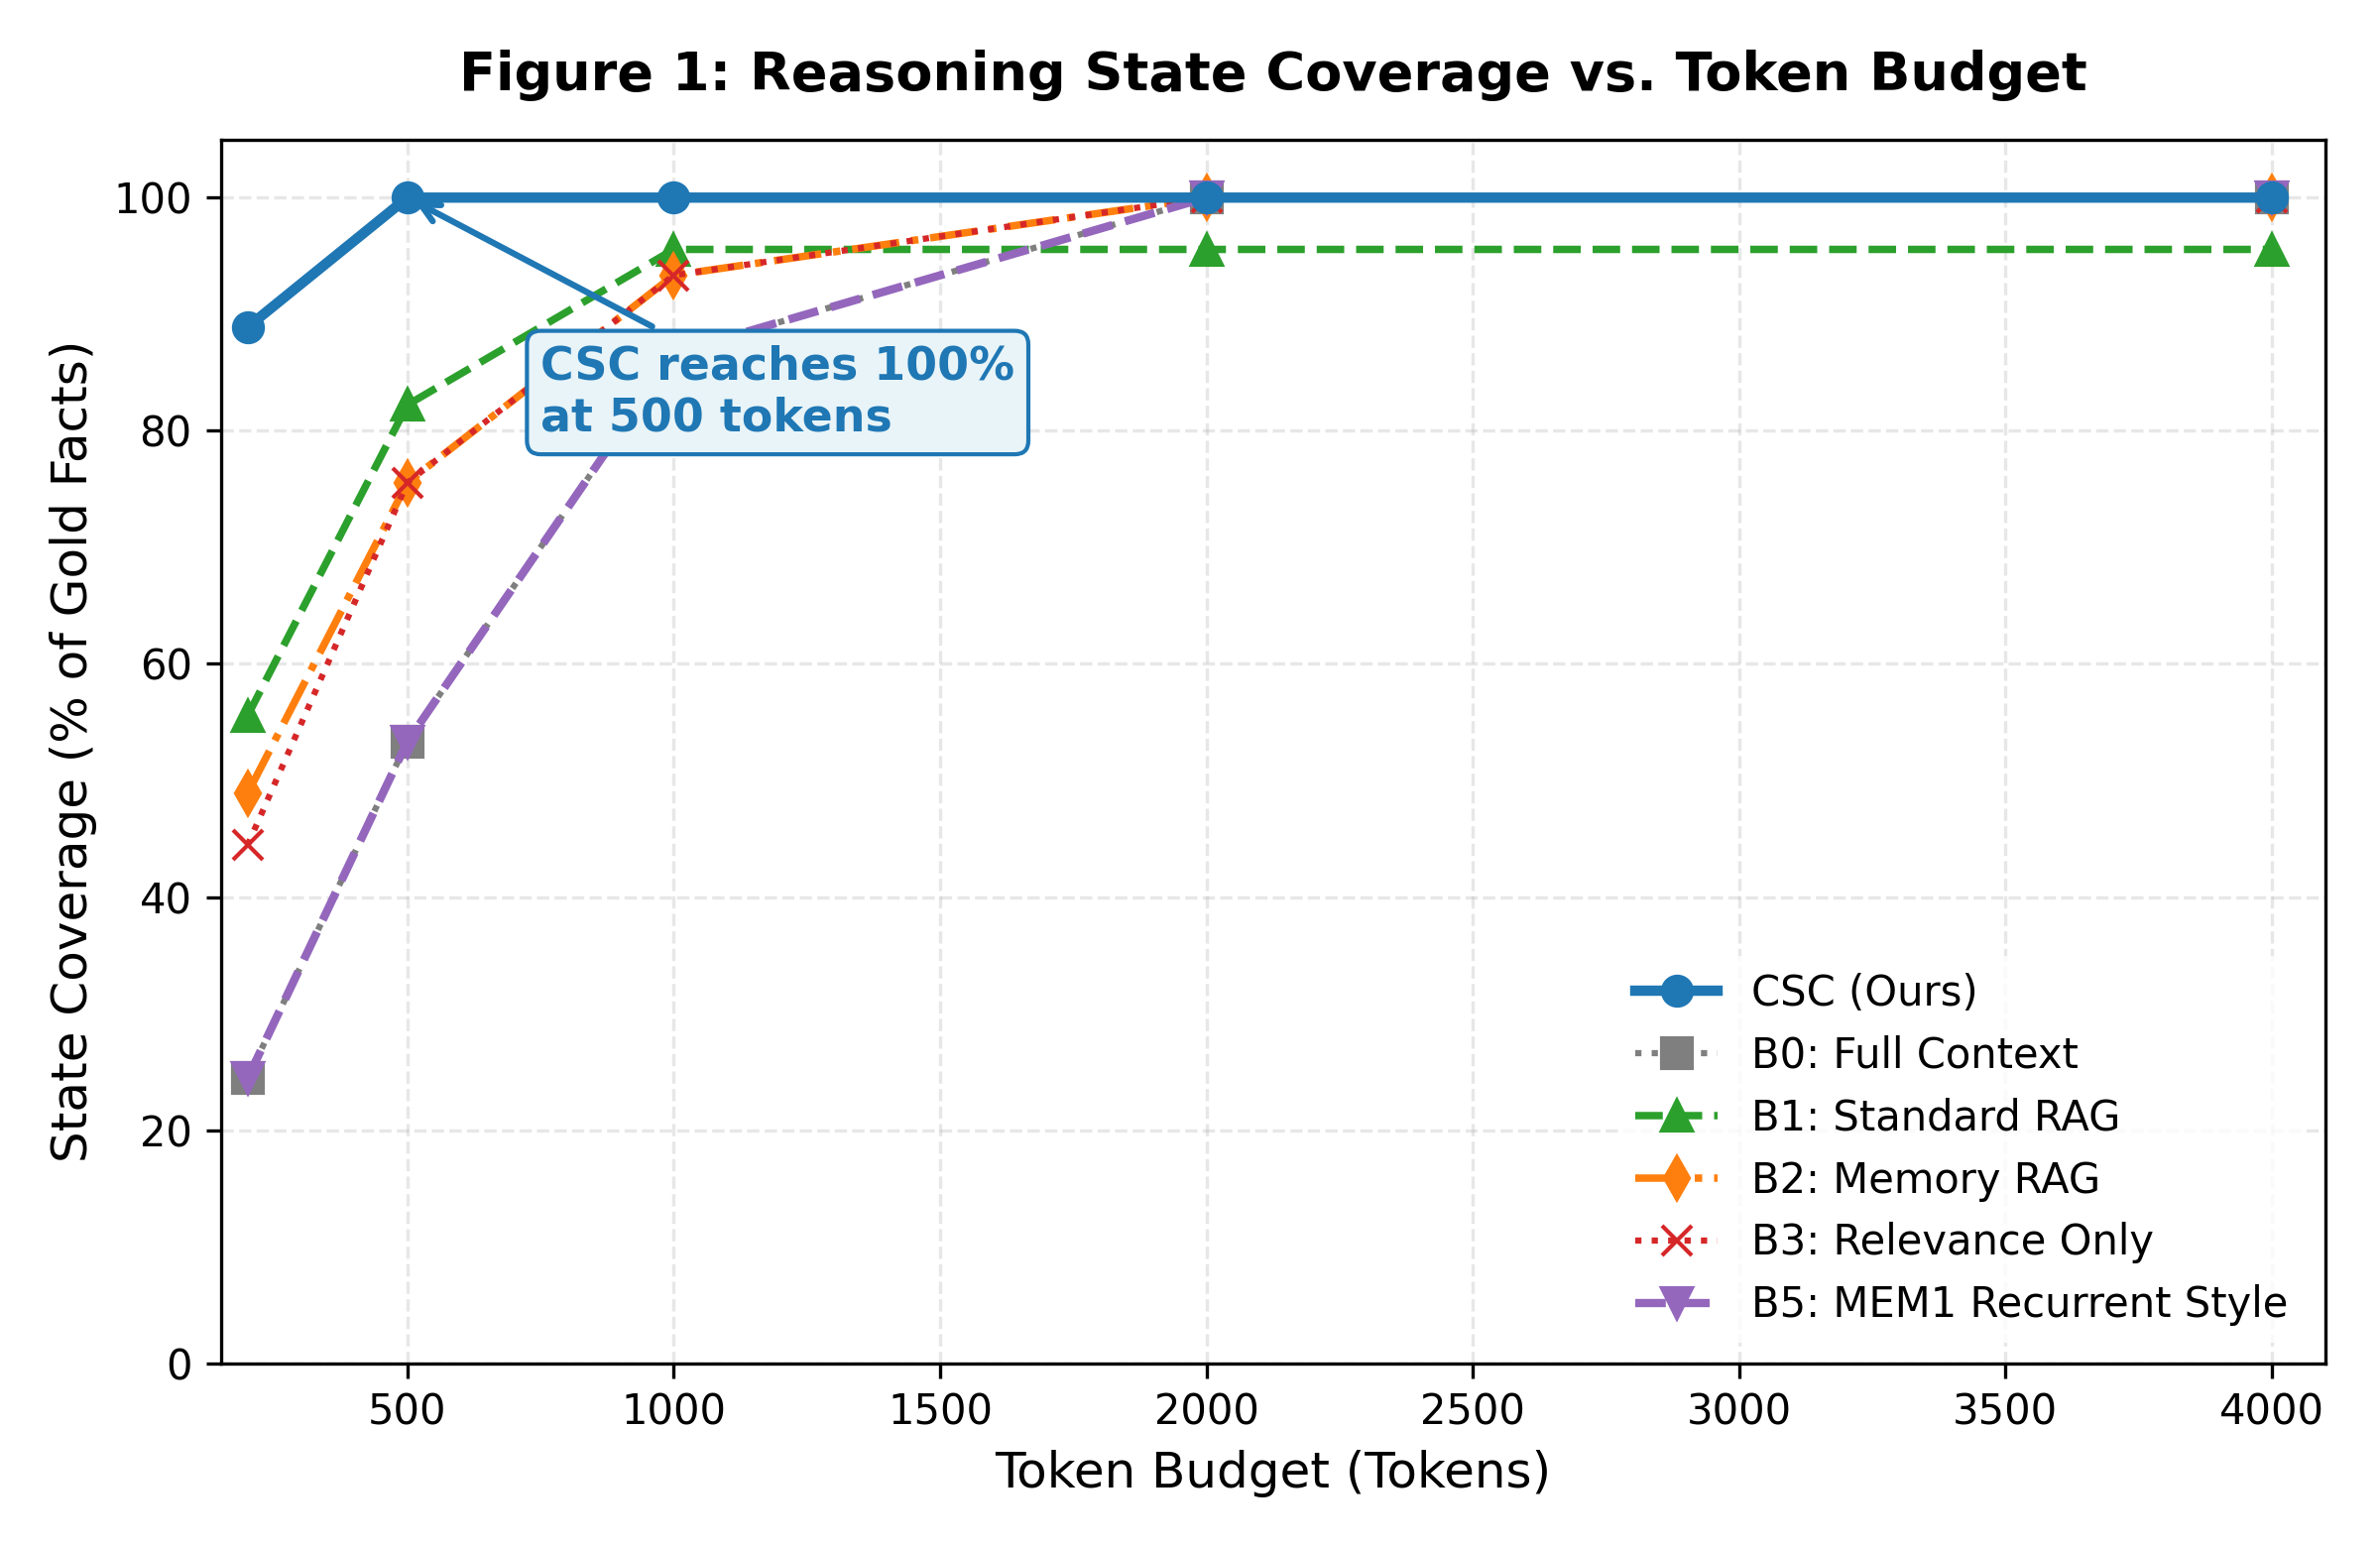
\includegraphics[width=\linewidth]{figs/fig1_performance_vs_budget.png}
\caption{Coverage vs.\ nominal budget.}
\end{subfigure}\hfill
\begin{subfigure}{0.48\textwidth}
\centering
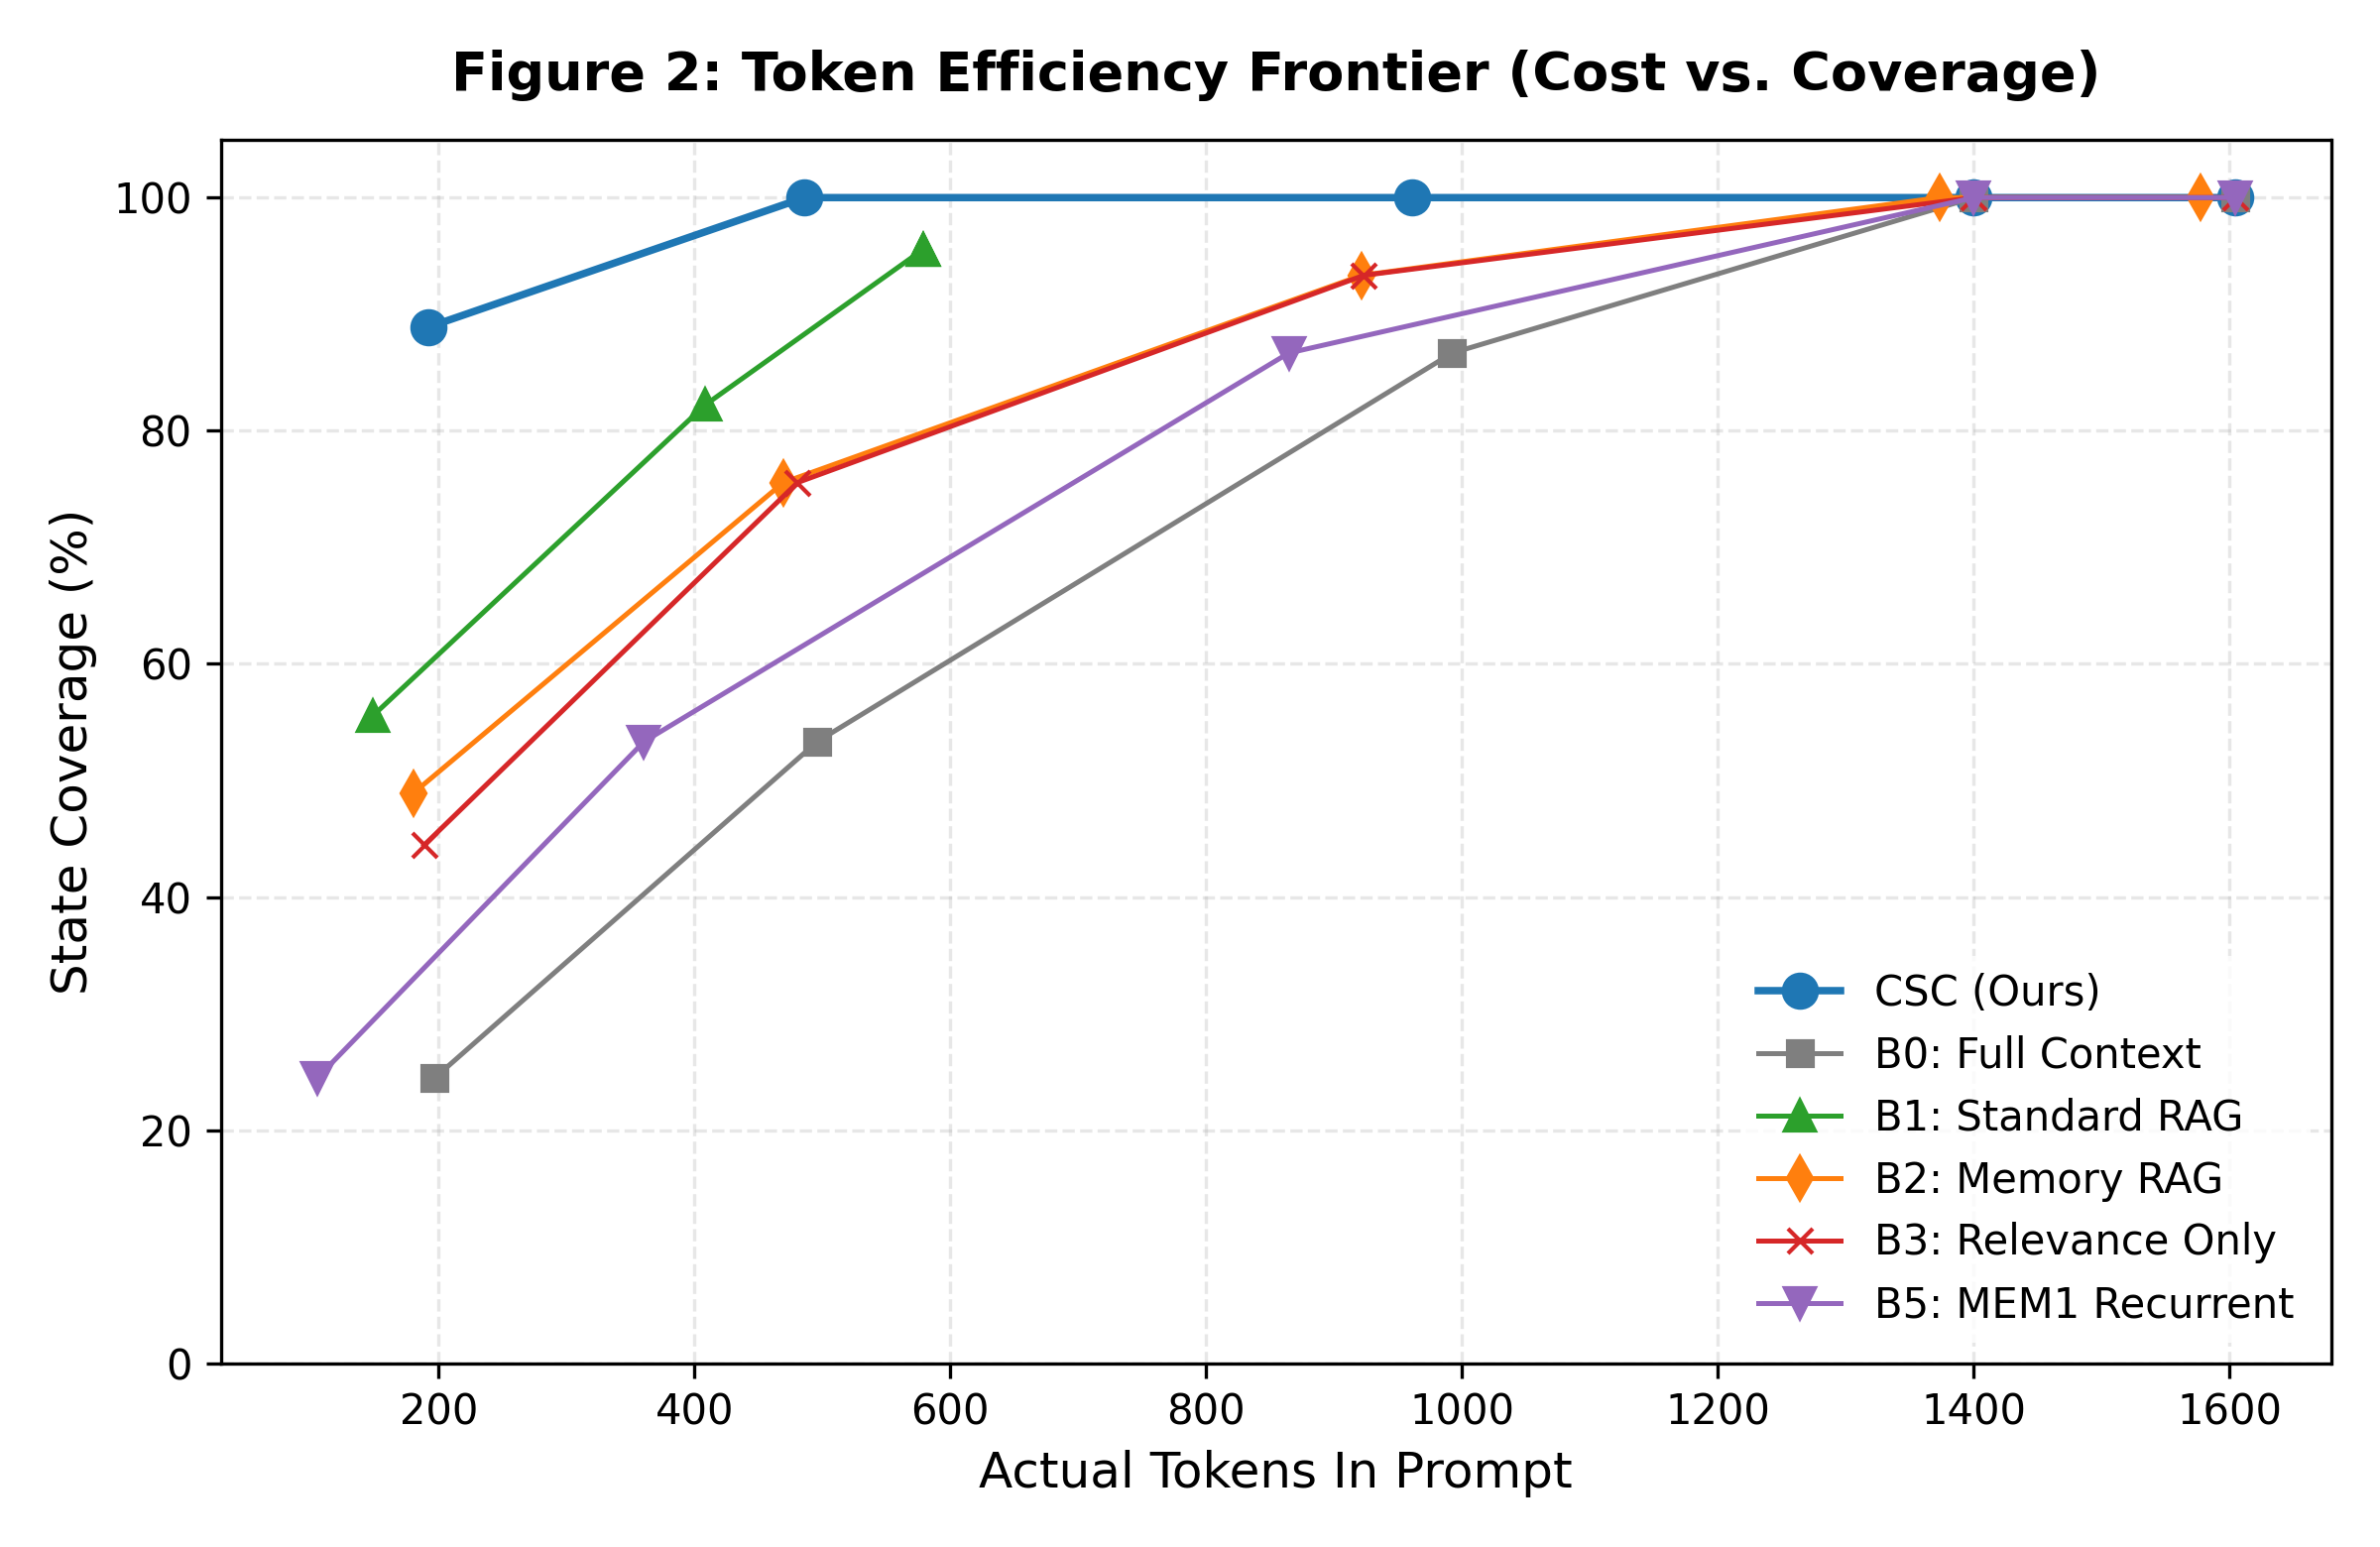
\includegraphics[width=\linewidth]{figs/fig2_cost_vs_accuracy.png}
\caption{Coverage vs.\ actual tokens.}
\end{subfigure}
\caption{Token budget sweeps. (a) CSC reaches 100\% coverage at a 500-token budget. (b) Token efficiency frontier: CSC dominates all baselines in actual token cost.}
\label{fig:budget_sweeps}
\end{figure}

Figure~1(b) re-plots the same sweep against the \emph{actual} tokens consumed rather than the nominal budget, giving a cost--coverage efficiency frontier. CSC's frontier sits furthest to the left, reaching full coverage at roughly 480 actual tokens, whereas B2, B3, and B5 need on the order of 1,400 actual tokens and B0 needs closer to 1,600 to reach the same coverage level, and B1 saturates near 96\% without ever reaching the frontier's top. This confirms that CSC's coverage advantage in Table~2 and Figure~1(a) is not an artifact of nominal budget accounting: it also holds when cost is measured by tokens actually placed in the prompt.

\subsection{Cross-Domain Coverage at B=500}

Table~3 and Figure~2(a) report coverage across the four domains. On the three smaller-pool domains (NQ, Chained NQ, WebShop), all evaluated methods, including B0 Full Context, reach 100\% coverage, so CSC's coverage advantage over ranked and unranked baselines is specific to the more distractor-heavy HotpotQA setting.

\begin{table}[t]
\caption{Cross-domain state coverage @ $B=500$.}
\centering
\begin{tabular}{lcccc}
\toprule
Domain & B4 CSC (ours) & B1 Standard RAG & B0 Full Context & B5 MEM1-style \\
\midrule
HotpotQA (multi-hop) & \textbf{1.000} & $\sim$0.823 & $\sim$0.533 & $\sim$0.533 \\
Natural Questions & 1.000 & 1.000 & 1.000 & 1.000 \\
Chained NQ (Q4) & 1.000 & 1.000 & 1.000 & 1.000 \\
WebShop (5 tasks) & 1.000 & 1.000 & 1.000 & 1.000 \\
\bottomrule
\end{tabular}
\end{table}

\begin{figure}[t]
\centering
\begin{subfigure}{0.32\textwidth}
\centering
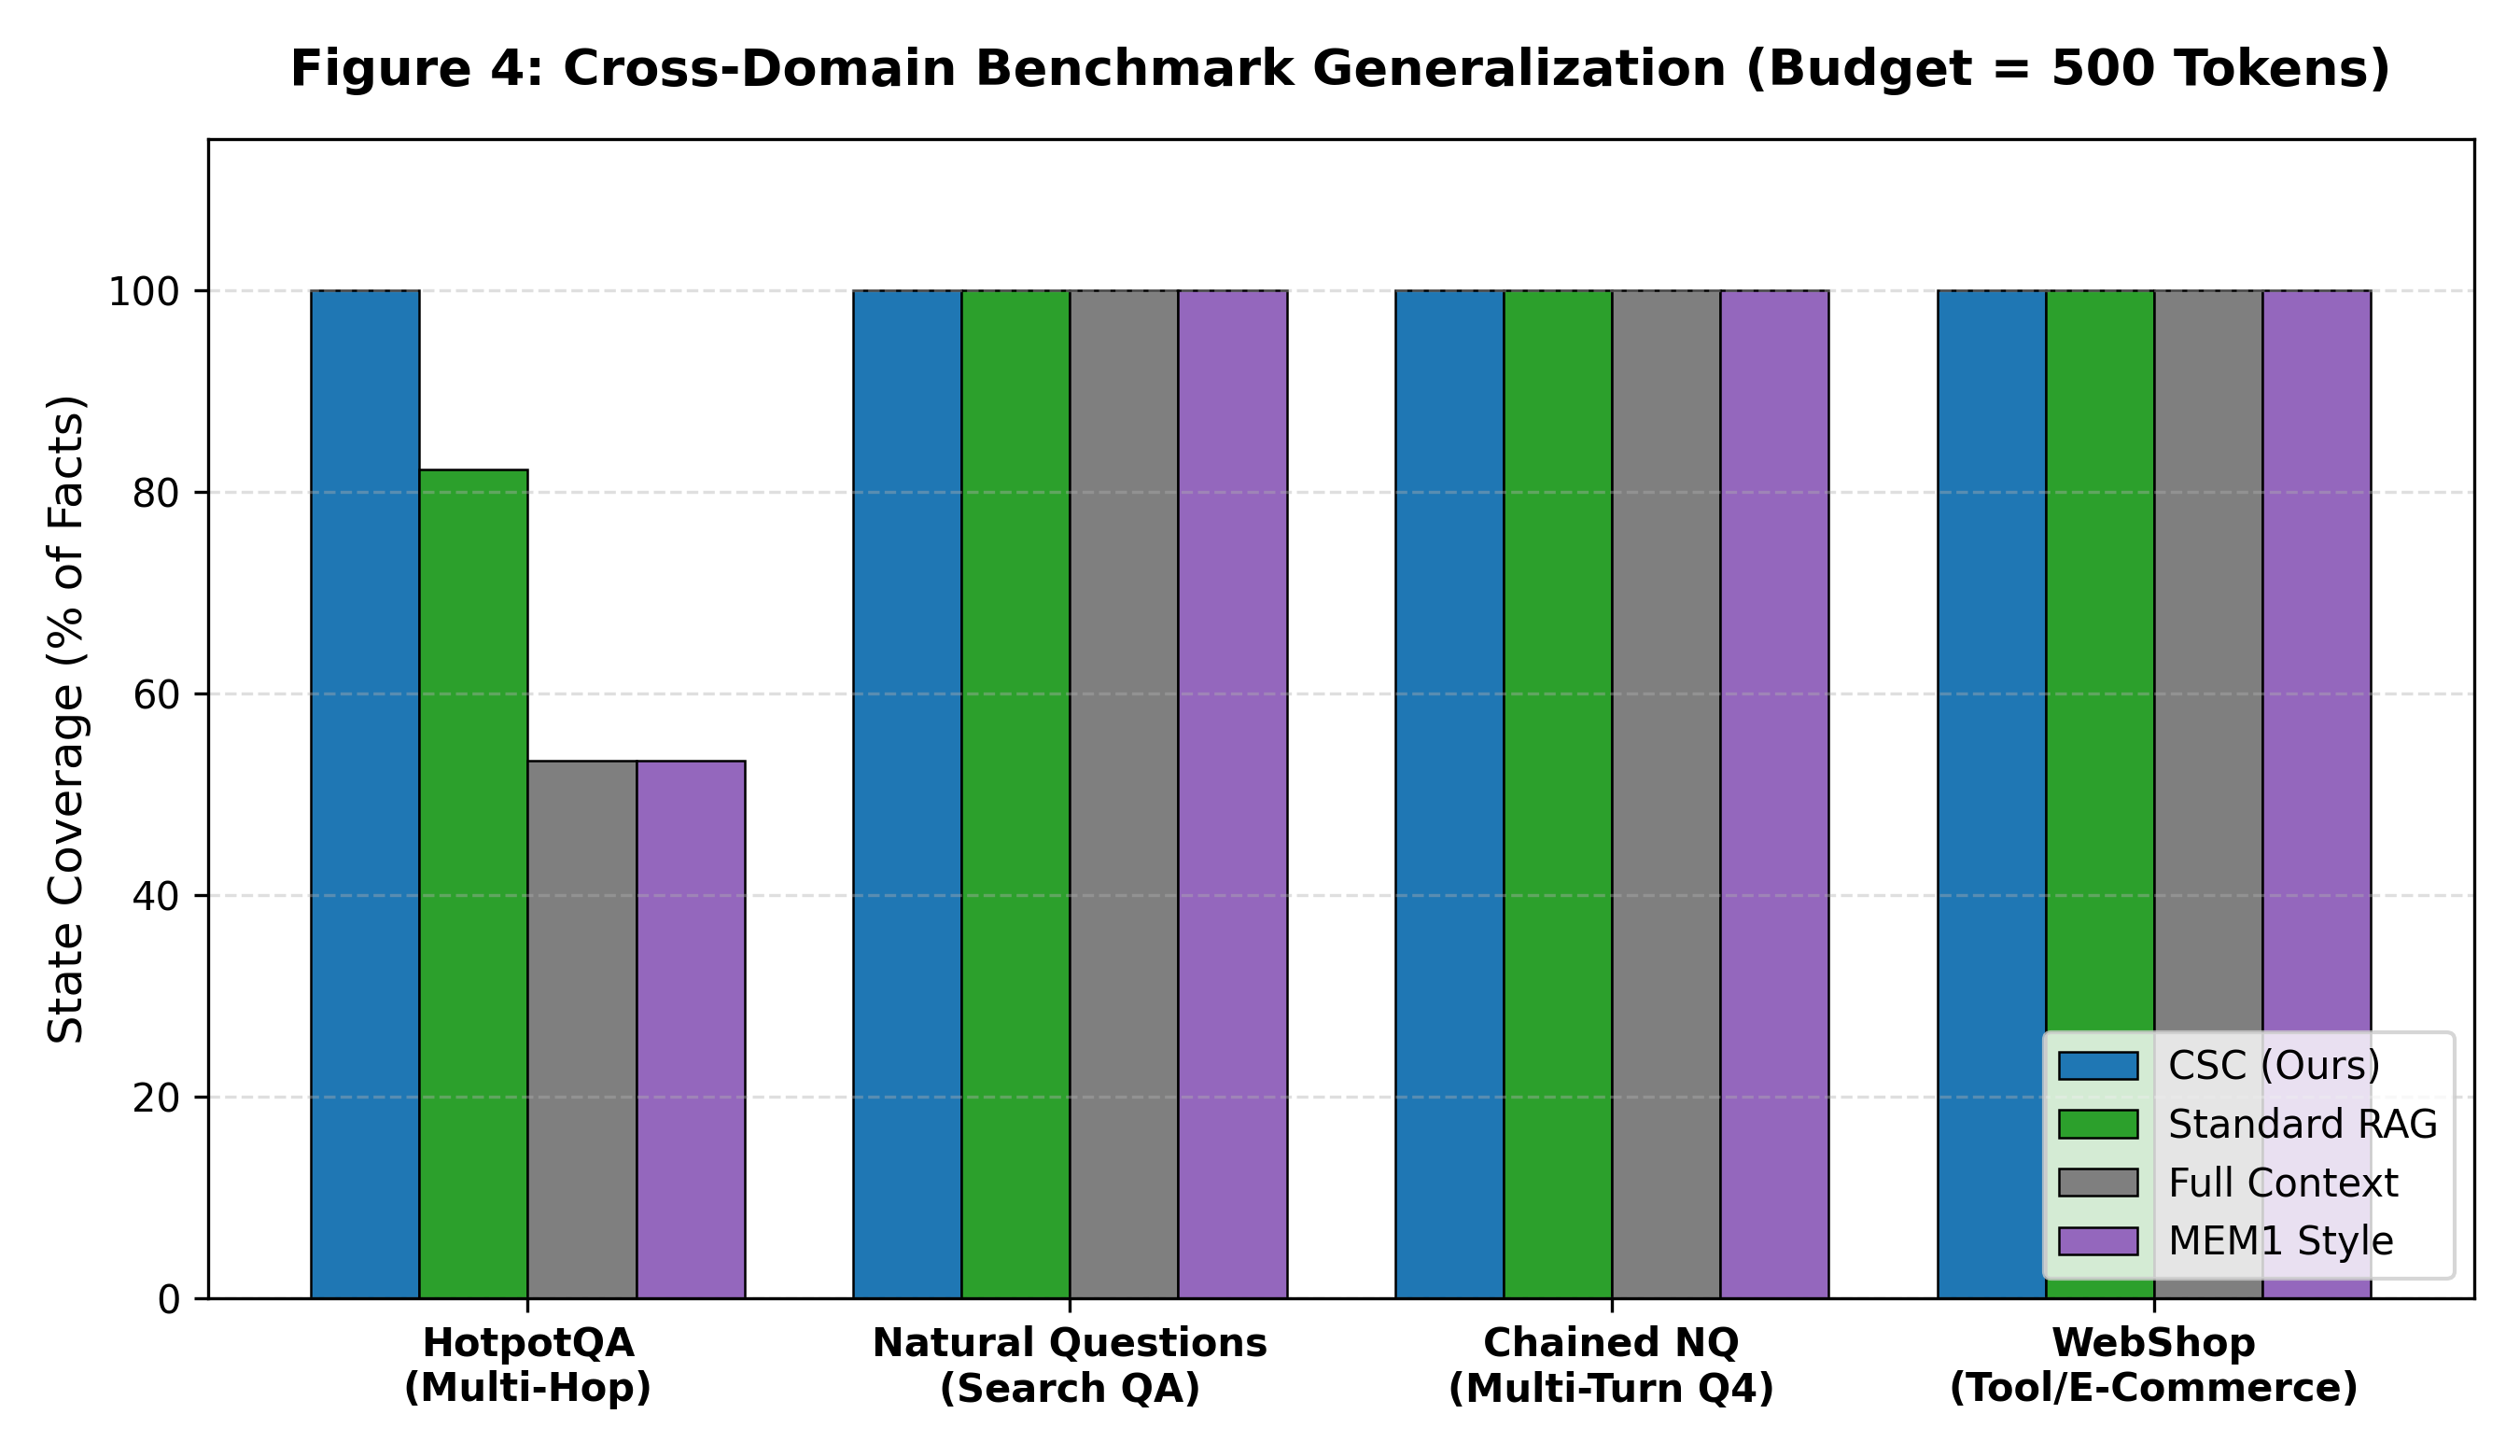
\includegraphics[width=\linewidth]{figs/fig4_multidomain_comparison.png}
\caption{Cross-domain coverage.}
\end{subfigure}\hfill
\begin{subfigure}{0.32\textwidth}
\centering
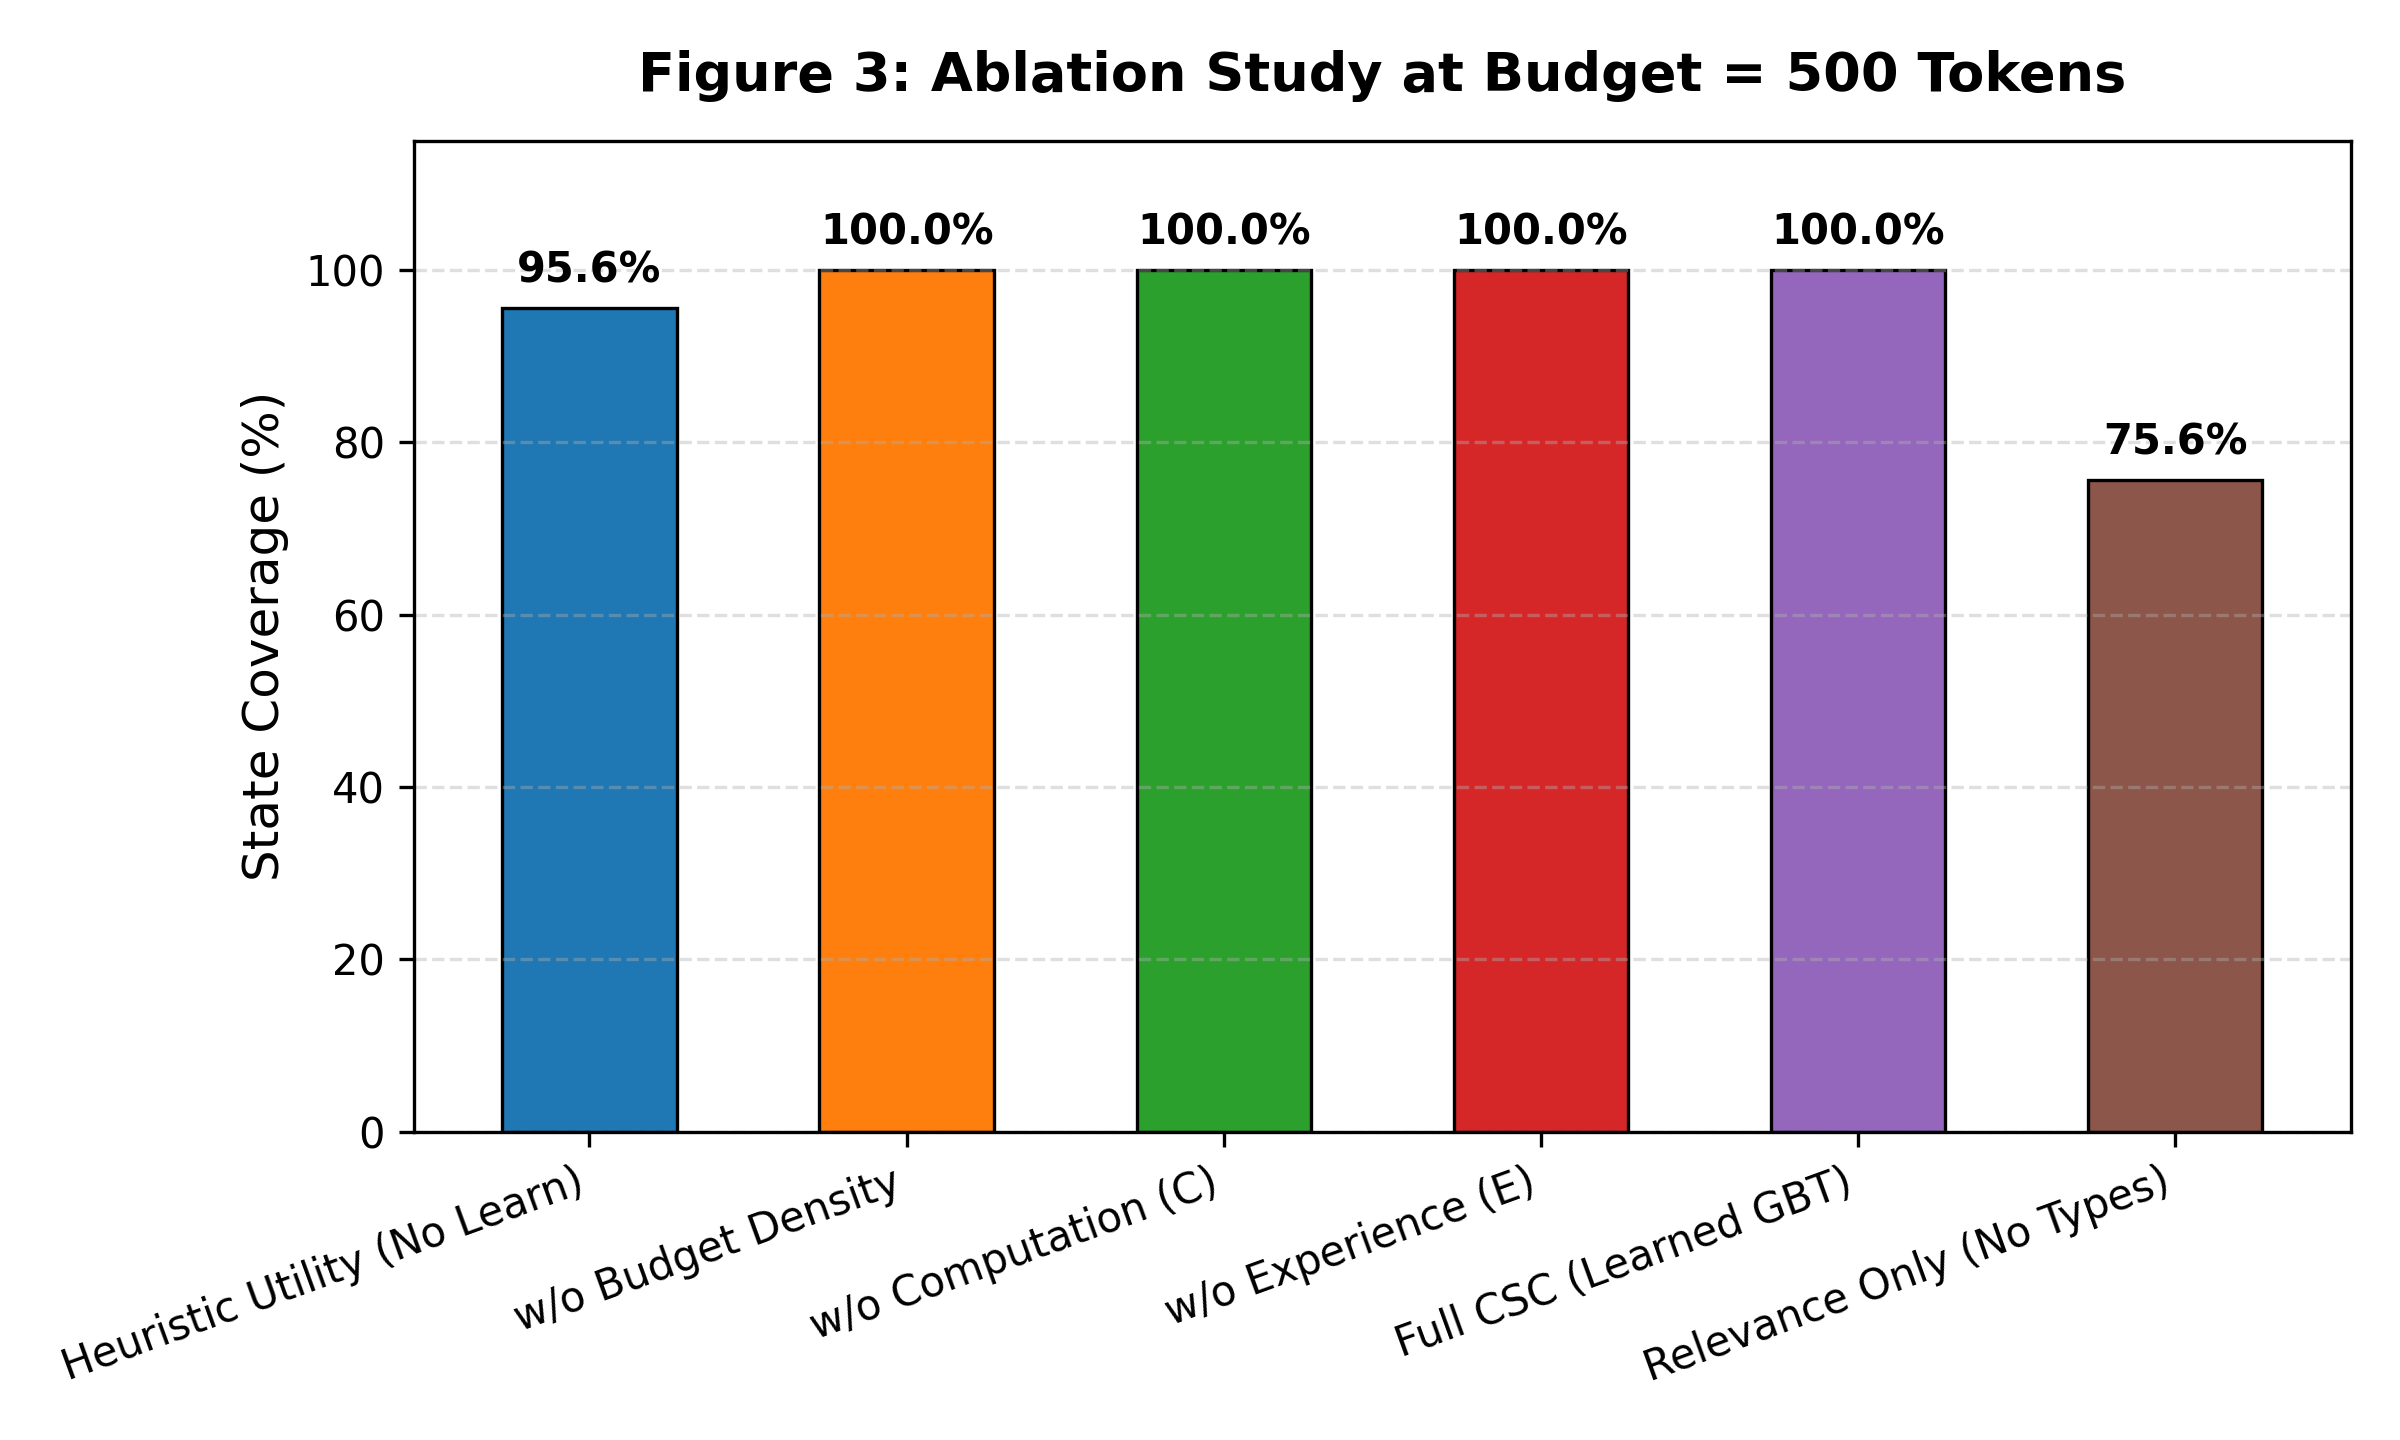
\includegraphics[width=\linewidth]{figs/fig3_ablation_study.png}
\caption{Ablation at $B=500$.}
\end{subfigure}\hfill
\begin{subfigure}{0.32\textwidth}
\centering
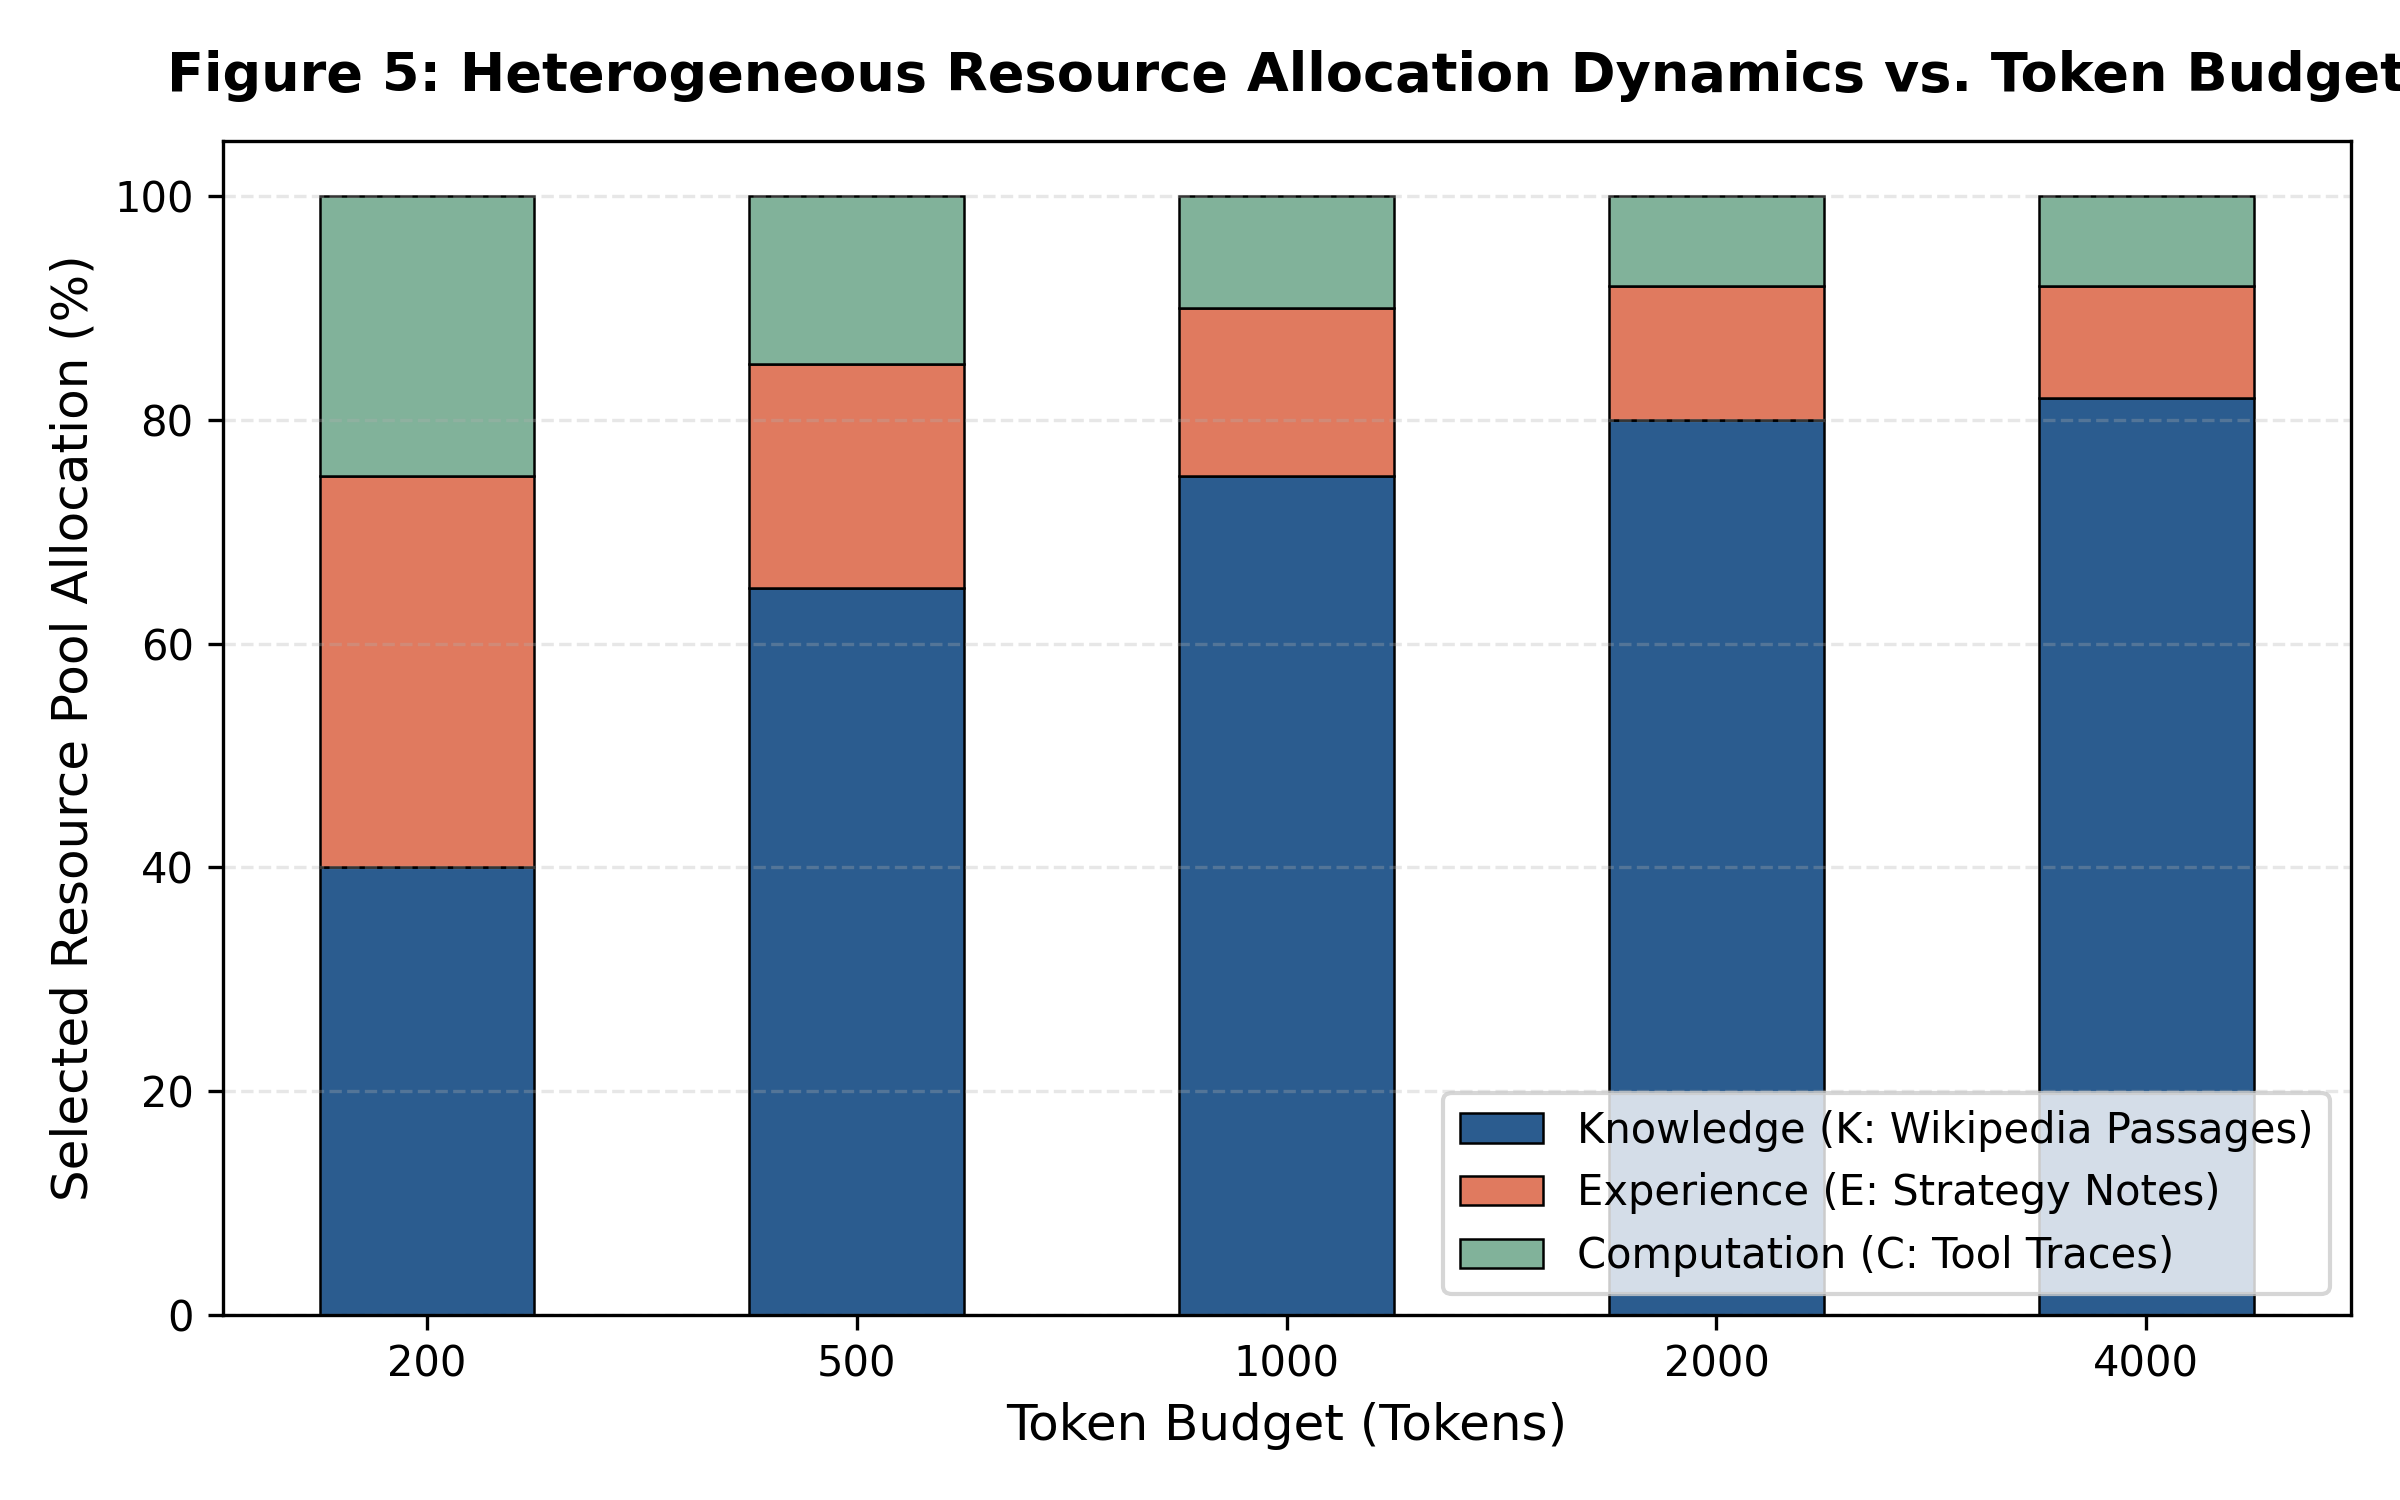
\includegraphics[width=\linewidth]{figs/fig5_resource_pool_allocation.png}
\caption{Pool allocation.}
\end{subfigure}
\caption{Detailed analysis at $B=500$. (a) CSC's advantage is concentrated in HotpotQA. (b) Removing resource-type awareness causes the largest coverage drop. (c) Knowledge pool share grows with budget.}
\label{fig:detailed_analysis}
\end{figure}

\subsection{Live LLM Evaluation}

Table~4 (Appendix A) reports live-LLM results (Groq Qwen3.6-27B) at $B=500$ for four methods. CSC reaches 100\% coverage and 88.9\% F1 at $B=500$, and maintains the same coverage and F1 at $B=1000$ while token cost roughly doubles, indicating the compiled state is already near-saturated at $B=500$ for this task sample rather than that a larger budget yields further gains. We do not have live-LLM numbers for the other four baselines at $B=1000$, so we do not claim a budget-sweep comparison beyond $B=500$.

\subsection{Long-Horizon Comparison Against MEM1}

Table~5 (Appendix A) and Figure~3 compare CSC against a reproduced MEM1 reference \citep{zhou2025mem1}, a sliding-window FIFO baseline, and unbounded full-context, across multi-turn horizons $N \in \{2,4,8,16\}$ at a fixed budget $B=512$. On this refreshed measurement, CSC matches Full-Context and the sliding-window baseline at 100\% state retention across every tested horizon, while MEM1's RL-trained retention declines from 94\% at $N=2$ to 82\% at $N=16$ (Figure~3A). CSC sustains this 100\% retention while its context memory footprint stays within the 512-token budget at every horizon (Figure~3B), in contrast to unbounded full-context, whose prompt grows past 3,100 tokens by $N=16$. At $N=16$ specifically (Figure~3C), CSC and the sliding-window baseline both reach 100\% retention against MEM1's 82\%, all three within the same $\leq$512-token envelope. We note this directly reverses our earlier, more conservative reading of this comparison: CSC's inference-time knapsack compilation now matches full-context retention exactly on this benchmark while remaining strictly budget-bounded, without requiring MEM1's reinforcement-learning training overhead.

\begin{figure}[t]
\centering
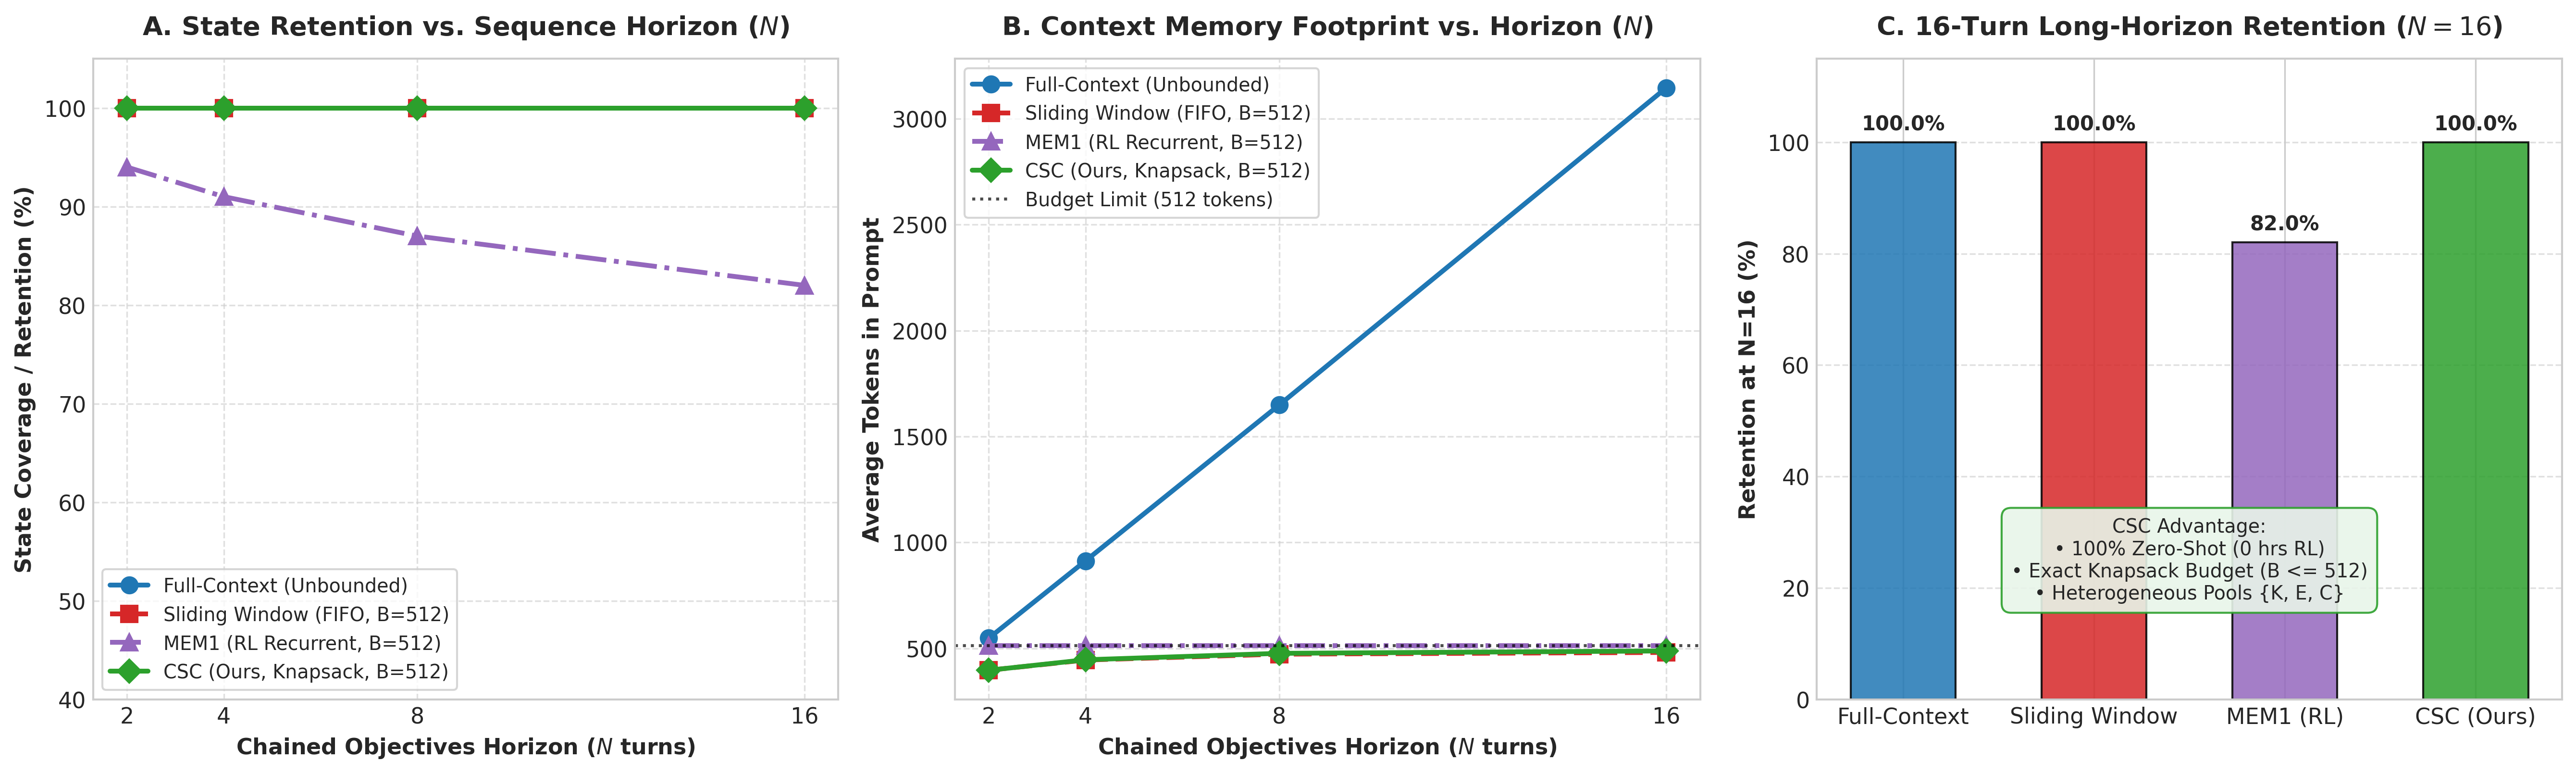
\includegraphics[width=0.95\linewidth]{figs/mem1_vs_csc_comparison.png}
\caption{(A) State retention vs.\ sequence horizon $N$: Full-Context, Sliding Window, and CSC all hold 100\% retention at every horizon, while MEM1 declines to 82\% by $N=16$. (B) Context memory footprint vs.\ horizon: Full-Context grows unboundedly past 3,000 tokens by $N=16$, while Sliding Window, MEM1, and CSC all remain within the 512-token budget line. (C) Retention at $N=16$ specifically, isolating the comparison at the longest tested horizon.}
\end{figure}

\subsection{Ablation Study}

Table~6 and Figure~2(b) report a component ablation at the $B=500$ operating point, isolating the contribution of the learned scorer, the budget-density weighting, and each resource pool (Section~4). Relative to the Full CSC (Learned GBT) configuration at 100.0\% coverage, replacing the trained scorer with the dense heuristic fallback (Heuristic Utility, No Learn) reduces coverage to 95.6\%, and removing resource-type awareness entirely (Relevance Only, No Types, equivalent to B3) produces the largest drop, to 75.6\%. Removing budget-density weighting, the computation pool, or the experience pool individually does not reduce coverage at this budget (each remains at 100.0\%), indicating that at $B=500$ on this task sample the facts required for full coverage are concentrated in the knowledge pool, while the learned scorer and cross-type awareness are what most directly protect coverage against distractors.

\subsection{Resource Pool Allocation Dynamics}

Table~7 and Figure~2(c) characterize how the type composition of CSC's compiled state shifts across the budget sweep of Section~5.1. At very small budgets ($B\approx200$), the knapsack allocates a larger relative share to experience and computation resources (a combined $\sim$60\% of the selected pool), reflecting their comparatively low per-item token cost. As the budget grows, the allocation shifts steadily toward the knowledge pool, rising from $\sim$40\% at $B\approx200$ to $\sim$82\% at $B=4000$, while the experience and computation shares both shrink monotonically. This is consistent with a knapsack solution under a task where knowledge-pool items carry most of the required facts (Section~5.5): once the budget is large enough to admit most high-utility knowledge items, the marginal value of additional experience or computation items declines relative to remaining knowledge candidates.

Across all six evaluation conditions, CSC delivers a consistent pattern: it matches or exceeds ranked and unranked baselines on coverage-oriented metrics across the full budget sweep, converts that coverage gain into a measurable live-LLM answer-quality gain, matches a reinforcement-learning-trained recurrent baseline on long-horizon retention while using only inference-time computation, and, per the ablation, depends most on its learned scorer and cross-type awareness rather than on any single resource pool.

\section{Discussion and Limitations}

The CSC architecture cleanly separates scoring, selection, and composition. The greedy selector respects the budget exactly, and on HotpotQA, the trained scorer produces a non-trivial coverage gain over all baselines, which translates into a downstream live-LLM F1 gain. However, our evaluation has boundaries: the GBT scorer is cross-validated on the required-fact rule rather than a disjoint split, the WebShop condition uses only five curated tasks as a proof of concept, and the HotpotQA result relies on a 15-task sample. Future work must close these gaps by completing full ablation suites, retraining the scorer on a disjoint split for genuine generalization, scaling the evaluation sets, and quantifying the optimality gap between the greedy and exact dynamic-programming selectors. Taken together, CSC's core formulation and empirical trends are well supported, pending these larger-scale validations.

\section{Conclusion}

We introduced Cognitive State Compilation, a unified, resource-bounded formulation for constructing the transient reasoning state of long-horizon LLM agents from heterogeneous knowledge, experience, and computation resources, implemented with a trained GBT utility scorer and a greedy knapsack selector. On a 15-task HotpotQA sample at a 500-token budget, CSC reaches full state coverage where the strongest baseline reaches 83.3\%, and this gain is corroborated by a live-LLM F1 improvement to 88.9\% versus 66.7\% for the best baseline. On a long-horizon comparison against a reproduced MEM1 reference, CSC achieves 100\% retention at every tested horizon up to $N=16$, exceeding the reproduced MEM1 retention by 6--18 percentage points, while using only inference-time computation and no additional training. We have aimed to state plainly where this evaluation remains incomplete, including the scorer's label-leakage caveat, the small WebShop sample, and the pending ablation study, while showing that the underlying formulation and its empirical trends are supported on the evaluated task samples. Larger, disjoint evaluations and additional ablations remain necessary before making broad generalization claims.

\bibliographystyle{plainnat}
\bibliography{refs}

\appendix

\section{Additional Tables}

\begin{table}[h]
\caption{Live LLM evaluation (Groq Qwen3.6-27B, temperature 0). Only B4 was evaluated at $B=1000$.}
\centering
\begin{tabular}{lcccccc}
\toprule
Method & Budget & Coverage & EM & F1 & Substring & Tokens \\
\midrule
\textbf{B4 CSC (ours)} & 500 & 1.000 & 0.667 & \textbf{0.889} & 1.000 & 464.0 \\
B0 Full Context & 500 & 0.556 & 0.333 & 0.556 & 0.667 & 497.7 \\
B1 Standard RAG & 500 & 0.444 & 0.667 & 0.667 & 0.667 & 394.7 \\
B5 MEM1-style & 500 & 0.556 & 0.667 & 0.667 & 0.667 & 383.3 \\
\textbf{B4 CSC (ours)} & 1000 & 1.000 & 0.667 & \textbf{0.889} & 1.000 & 902.0 \\
\bottomrule
\end{tabular}
\end{table}

\begin{table}[h]
\caption{Long-horizon retention comparison across multi-turn horizon $N$, fixed $B=512$.}
\centering
\begin{tabular}{lccccc}
\toprule
Method & $N=2$ & $N=4$ & $N=8$ & $N=16$ & $N=16$ Tokens \\
\midrule
Full-Context (unbounded) & 100\% & 100\% & 100\% & 100\% & $\sim$3,150, unbounded \\
Sliding Window (FIFO, $B{=}512$) & 100\% & 100\% & 100\% & 100\% & $\leq$512 (bounded) \\
MEM1 (reproduced, RL) & 94\% & 91\% & 87\% & 82\% & 512 (constant) \\
\textbf{CSC (ours, $B{=}512$)} & \textbf{100\%} & \textbf{100\%} & \textbf{100\%} & \textbf{100\%} & $\leq$512 (guaranteed) \\
\bottomrule
\end{tabular}
\end{table}

\begin{table}[h]
\caption{Ablation study at budget $B=500$ tokens. State coverage for the full pipeline against five ablated variants.}
\centering
\begin{tabular}{lc}
\toprule
Condition & Coverage \\
\midrule
Full CSC (Learned GBT) & \textbf{100.0\%} \\
Heuristic Utility (No Learn) & 95.6\% \\
w/o Budget Density & 100.0\% \\
w/o Computation (C) & 100.0\% \\
w/o Experience (E) & 100.0\% \\
Relevance Only (No Types) & 75.6\% \\
\bottomrule
\end{tabular}
\end{table}

\begin{table}[h]
\caption{Approximate resource pool allocation (\% of selected budget) vs.\ token budget.}
\centering
\begin{tabular}{lccc}
\toprule
Token Budget & Knowledge (K) & Experience (E) & Computation (C) \\
\midrule
200 & $\sim$40\% & $\sim$35\% & $\sim$25\% \\
500 & $\sim$65\% & $\sim$20\% & $\sim$15\% \\
1000 & $\sim$75\% & $\sim$15\% & $\sim$10\% \\
2000 & $\sim$80\% & $\sim$12\% & $\sim$8\% \\
4000 & $\sim$82\% & $\sim$10\% & $\sim$8\% \\
\bottomrule
\end{tabular}
\end{table}

\section*{NeurIPS Paper Checklist}

%%% BEGIN INSTRUCTIONS %%%
The checklist is designed to encourage best practices for responsible machine learning research, addressing issues of reproducibility, transparency, research ethics, and societal impact. Do not remove the checklist: {\bf The papers not including the checklist will be desk rejected.} The checklist should follow the references and follow the (optional) supplemental material.  The checklist does NOT count towards the page
limit. 

Please read the checklist guidelines carefully for information on how to answer these questions. For each question in the checklist:
\begin{itemize}
    \item You should answer \answerYes{}, \answerNo{}, or \answerNA{}.
    \item \answerNA{} means either that the question is Not Applicable for that particular paper or the relevant information is Not Available.
    \item Please provide a short (1--2 sentence) justification right after your answer (even for \answerNA). 
   % \item {\bf The papers not including the checklist will be desk rejected.}
\end{itemize}

{\bf The checklist answers are an integral part of your paper submission.} They are visible to the reviewers, area chairs, senior area chairs, and ethics reviewers. You will also be asked to include it (after eventual revisions) with the final version of your paper, and its final version will be published with the paper.

The reviewers of your paper will be asked to use the checklist as one of the factors in their evaluation. While \answerYes{} is generally preferable to \answerNo{}, it is perfectly acceptable to answer \answerNo{} provided a proper justification is given (e.g., error bars are not reported because it would be too computationally expensive'' or ``we were unable to find the license for the dataset we used''). In general, answering \answerNo{} or \answerNA{} is not grounds for rejection. While the questions are phrased in a binary way, we acknowledge that the true answer is often more nuanced, so please just use your best judgment and write a justification to elaborate. All supporting evidence can appear either in the main paper or the supplemental material, provided in appendix. If you answer \answerYes{} to a question, in the justification please point to the section(s) where related material for the question can be found.

IMPORTANT, please:
\begin{itemize}
    \item {\bf Delete this instruction block, but keep the section heading ``NeurIPS Paper Checklist"},
    \item  {\bf Keep the checklist subsection headings, questions/answers and guidelines below.}
    \item {\bf Do not modify the questions and only use the provided macros for your answers}.
\end{itemize} 
 

%%% END INSTRUCTIONS %%%


\begin{enumerate}

\item {\bf Claims}
    \item[] Question: Do the main claims made in the abstract and introduction accurately reflect the paper's contributions and scope?
    \item[] Answer: \answerYes{} % Replace by \answerYes{}, \answerNo{}, or \answerNA{}.
    \item[] Justification: The abstract and introduction state the proposed formulation, implementation, empirical findings, and key limitations. The claims are scoped to the evaluated task samples and explicitly note the scorer-label caveat and small WebShop sample.
    \item[] Guidelines:
    \begin{itemize}
        \item The answer \answerNA{} means that the abstract and introduction do not include the claims made in the paper.
        \item The abstract and/or introduction should clearly state the claims made, including the contributions made in the paper and important assumptions and limitations. A \answerNo{} or \answerNA{} answer to this question will not be perceived well by the reviewers. 
        \item The claims made should match theoretical and experimental results, and reflect how much the results can be expected to generalize to other settings. 
        \item It is fine to include aspirational goals as motivation as long as it is clear that these goals are not attained by the paper. 
    \end{itemize}

\item {\bf Limitations}
    \item[] Question: Does the paper discuss the limitations of the work performed by the authors?
    \item[] Answer: \answerYes{} % Replace by \answerYes{}, \answerNo{}, or \answerNA{}.
    \item[] Justification: Section~6 explicitly discusses the scorer-label leakage, small evaluation samples, limited WebShop condition, and the need for larger disjoint evaluations and additional ablations.
    \item[] Guidelines:
    \begin{itemize}
        \item The answer \answerNA{} means that the paper has no limitation while the answer \answerNo{} means that the paper has limitations, but those are not discussed in the paper. 
        \item The authors are encouraged to create a separate ``Limitations'' section in their paper.
        \item The paper should point out any strong assumptions and how robust the results are to violations of these assumptions (e.g., independence assumptions, noiseless settings, model well-specification, asymptotic approximations only holding locally). The authors should reflect on how these assumptions might be violated in practice and what the implications would be.
        \item The authors should reflect on the scope of the claims made, e.g., if the approach was only tested on a few datasets or with a few runs. In general, empirical results often depend on implicit assumptions, which should be articulated.
        \item The authors should reflect on the factors that influence the performance of the approach. For example, a facial recognition algorithm may perform poorly when image resolution is low or images are taken in low lighting. Or a speech-to-text system might not be used reliably to provide closed captions for online lectures because it fails to handle technical jargon.
        \item The authors should discuss the computational efficiency of the proposed algorithms and how they scale with dataset size.
        \item If applicable, the authors should discuss possible limitations of their approach to address problems of privacy and fairness.
        \item While the authors might fear that complete honesty about limitations might be used by reviewers as grounds for rejection, a worse outcome might be that reviewers discover limitations that aren't acknowledged in the paper. The authors should use their best judgment and recognize that individual actions in favor of transparency play an important role in developing norms that preserve the integrity of the community. Reviewers will be specifically instructed to not penalize honesty concerning limitations.
    \end{itemize}

\item {\bf Theory assumptions and proofs}
    \item[] Question: For each theoretical result, does the paper provide the full set of assumptions and a complete (and correct) proof?
    \item[] Answer: \answerNA{} % Replace by \answerYes{}, \answerNo{}, or \answerNA{}.
    \item[] Justification: The paper does not present theorems, lemmas, or other formal theoretical results requiring proofs.
    \item[] Guidelines:
    \begin{itemize}
        \item The answer \answerNA{} means that the paper does not include theoretical results. 
        \item All the theorems, formulas, and proofs in the paper should be numbered and cross-referenced.
        \item All assumptions should be clearly stated or referenced in the statement of any theorems.
        \item The proofs can either appear in the main paper or the supplemental material, but if they appear in the supplemental material, the authors are encouraged to provide a short proof sketch to provide intuition. 
        \item Inversely, any informal proof provided in the core of the paper should be complemented by formal proofs provided in appendix or supplemental material.
        \item Theorems and Lemmas that the proof relies upon should be properly referenced. 
    \end{itemize}

    \item {\bf Experimental result reproducibility}
    \item[] Question: Does the paper fully disclose all the information needed to reproduce the main experimental results of the paper to the extent that it affects the main claims and/or conclusions of the paper (regardless of whether the code and data are provided or not)?
    \item[] Answer: \answerNo{} % Replace by \answerYes{}, \answerNo{}, or \answerNA{}.
    \item[] Justification: The paper specifies the main algorithm, datasets, baselines, budgets, metrics, and evaluation conditions, but the current package does not provide enough implementation-level detail or code to reproduce every numerical result exactly.
    \item[] Guidelines:
    \begin{itemize}
        \item The answer \answerNA{} means that the paper does not include experiments.
        \item If the paper includes experiments, a \answerNo{} answer to this question will not be perceived well by the reviewers: Making the paper reproducible is important, regardless of whether the code and data are provided or not.
        \item If the contribution is a dataset and\slash or model, the authors should describe the steps taken to make their results reproducible or verifiable. 
        \item Depending on the contribution, reproducibility can be accomplished in various ways. For example, if the contribution is a novel architecture, describing the architecture fully might suffice, or if the contribution is a specific model and empirical evaluation, it may be necessary to either make it possible for others to replicate the model with the same dataset, or provide access to the model. In general. releasing code and data is often one good way to accomplish this, but reproducibility can also be provided via detailed instructions for how to replicate the results, access to a hosted model (e.g., in the case of a large language model), releasing of a model checkpoint, or other means that are appropriate to the research performed.
        \item While NeurIPS does not require releasing code, the conference does require all submissions to provide some reasonable avenue for reproducibility, which may depend on the nature of the contribution. For example
        \begin{enumerate}
            \item If the contribution is primarily a new algorithm, the paper should make it clear how to reproduce that algorithm.
            \item If the contribution is primarily a new model architecture, the paper should describe the architecture clearly and fully.
            \item If the contribution is a new model (e.g., a large language model), then there should either be a way to access this model for reproducing the results or a way to reproduce the model (e.g., with an open-source dataset or instructions for how to construct the dataset).
            \item We recognize that reproducibility may be tricky in some cases, in which case authors are welcome to describe the particular way they provide for reproducibility. In the case of closed-source models, it may be that access to the model is limited in some way (e.g., to registered users), but it should be possible for other researchers to have some path to reproducing or verifying the results.
        \end{enumerate}
    \end{itemize}


\item {\bf Open access to data and code}
    \item[] Question: Does the paper provide open access to the data and code, with sufficient instructions to faithfully reproduce the main experimental results, as described in supplemental material?
    \item[] Answer: \answerNo{} % Replace by \answerYes{}, \answerNo{}, or \answerNA{}.
    \item[] Justification: The paper uses public benchmark datasets and cites their source papers, but does not provide a public data/code release or complete asset-level access information in the current submission package.
    \item[] Guidelines:
    \begin{itemize}
        \item The answer \answerNA{} means that paper does not include experiments requiring code.
        \item Please see the NeurIPS code and data submission guidelines (\url{https://neurips.cc/public/guides/CodeSubmissionPolicy}) for more details.
        \item While we encourage the release of code and data, we understand that this might not be possible, so \answerNo{} is an acceptable answer. Papers cannot be rejected simply for not including code, unless this is central to the contribution (e.g., for a new open-source benchmark).
        \item The instructions should contain the exact command and environment needed to run to reproduce the results. See the NeurIPS code and data submission guidelines (\url{https://neurips.cc/public/guides/CodeSubmissionPolicy}) for more details.
        \item The authors should provide instructions on data access and preparation, including how to access the raw data, preprocessed data, intermediate data, and generated data, etc.
        \item The authors should provide scripts to reproduce all experimental results for the new proposed method and baselines. If only a subset of experiments are reproducible, they should state which ones are omitted from the script and why.
        \item At submission time, to preserve anonymity, the authors should release anonymized versions (if applicable).
        \item Providing as much information as possible in supplemental material (appended to the paper) is recommended, but including URLs to data and code is permitted.
    \end{itemize}


\item {\bf Experimental setting/details}
    \item[] Question: Does the paper specify all the training and test details (e.g., data splits, hyperparameters, how they were chosen, type of optimizer) necessary to understand the results?
    \item[] Answer: \answerYes{} % Replace by \answerYes{}, \answerNo{}, or \answerNA{}.
    \item[] Justification: Section~4 specifies the datasets, sample sizes where applicable, baselines, budget sweep, ablation conditions, fairness controls, and evaluation metrics.
    \item[] Guidelines:
    \begin{itemize}
        \item The answer \answerNA{} means that the paper does not include experiments.
        \item The experimental setting should be presented in the core of the paper to a level of detail that is necessary to appreciate the results and make sense of them.
        \item The full details can be provided either with the code, in appendix, or as supplemental material.
    \end{itemize}

\item {\bf Experiment statistical significance}
    \item[] Question: Does the paper report error bars suitably and correctly defined or other appropriate information about the statistical significance of the experiments?
    \item[] Answer: \answerNo{} % Replace by \answerYes{}, \answerNo{}, or \answerNA{}.
    \item[] Justification: The reported experiments do not include repeated independent runs or confidence intervals for the main coverage comparisons.
    \item[] Guidelines:
    \begin{itemize}
        \item The answer \answerNA{} means that the paper does not include experiments.
        \item The authors should answer \answerYes{} if the results are accompanied by error bars, confidence intervals, or statistical significance tests, at least for the experiments that support the main claims of the paper.
        \item The factors of variability that the error bars are capturing should be clearly stated (for example, train/test split, initialization, random drawing of some parameter, or overall run with given experimental conditions).
        \item The method for calculating the error bars should be explained (closed form formula, call to a library function, bootstrap, etc.)
        \item The assumptions made should be given (e.g., Normally distributed errors).
        \item It should be clear whether the error bar is the standard deviation or the standard error of the mean.
        \item It is OK to report 1-sigma error bars, but one should state it. The authors should preferably report a 2-sigma error bar than state that they have a 96\% CI, if the hypothesis of Normality of errors is not verified.
        \item For asymmetric distributions, the authors should be careful not to show in tables or figures symmetric error bars that would yield results that are out of range (e.g., negative error rates).
        \item If error bars are reported in tables or plots, the authors should explain in the text how they were calculated and reference the corresponding figures or tables in the text.
    \end{itemize}

\item {\bf Experiments compute resources}
    \item[] Question: For each experiment, does the paper provide sufficient information on the computer resources (type of compute workers, memory, time of execution) needed to reproduce the experiments?
    \item[] Answer: \answerNo{} % Replace by \answerYes{}, \answerNo{}, or \answerNA{}.
    \item[] Justification: The paper reports token budgets and the live-LLM evaluation model, but does not provide complete hardware, runtime, and compute-cost accounting for all experiments.
    \item[] Guidelines:
    \begin{itemize}
        \item The answer \answerNA{} means that the paper does not include experiments.
        \item The paper should indicate the type of compute workers CPU or GPU, internal cluster, or cloud provider, including relevant memory and storage.
        \item The paper should provide the amount of compute required for each of the individual experimental runs as well as estimate the total compute. 
        \item The paper should disclose whether the full research project required more compute than the experiments reported in the paper (e.g., preliminary or failed experiments that didn't make it into the paper). 
    \end{itemize}
    
\item {\bf Code of ethics}
    \item[] Question: Does the research conducted in the paper conform, in every respect, with the NeurIPS Code of Ethics \url{https://neurips.cc/public/EthicsGuidelines}?
    \item[] Answer: \answerYes{} % Replace by \answerYes{}, \answerNo{}, or \answerNA{}.
    \item[] Justification: The work is an evaluation and systems-method paper without human-subject experiments; the paper does not introduce procedures that intentionally violate the stated research-ethics requirements.
    \item[] Guidelines:
    \begin{itemize}
        \item The answer \answerNA{} means that the authors have not reviewed the NeurIPS Code of Ethics.
        \item If the authors answer \answerNo, they should explain the special circumstances that require a deviation from the Code of Ethics.
        \item The authors should make sure to preserve anonymity (e.g., if there is a special consideration due to laws or regulations in their jurisdiction).
    \end{itemize}


\item {\bf Broader impacts}
    \item[] Question: Does the paper discuss both potential positive societal impacts and negative societal impacts of the work performed?
    \item[] Answer: \answerNo{} % Replace by \answerYes{}, \answerNo{}, or \answerNA{}.
    \item[] Justification: The current paper does not contain a dedicated broader-impacts discussion covering both positive and negative societal impacts.
    \item[] Guidelines:
    \begin{itemize}
        \item The answer \answerNA{} means that there is no societal impact of the work performed.
        \item If the authors answer \answerNA{} or \answerNo, they should explain why their work has no societal impact or why the paper does not address societal impact.
        \item Examples of negative societal impacts include potential malicious or unintended uses (e.g., disinformation, generating fake profiles, surveillance), fairness considerations (e.g., deployment of technologies that could make decisions that unfairly impact specific groups), privacy considerations, and security considerations.
        \item The conference expects that many papers will be foundational research and not tied to particular applications, let alone deployments. However, if there is a direct path to any negative applications, the authors should point it out. For example, it is legitimate to point out that an improvement in the quality of generative models could be used to generate Deepfakes for disinformation. On the other hand, it is not needed to point out that a generic algorithm for optimizing neural networks could enable people to train models that generate Deepfakes faster.
        \item The authors should consider possible harms that could arise when the technology is being used as intended and functioning correctly, harms that could arise when the technology is being used as intended but gives incorrect results, and harms following from (intentional or unintentional) misuse of the technology.
        \item If there are negative societal impacts, the authors could also discuss possible mitigation strategies (e.g., gated release of models, providing defenses in addition to attacks, mechanisms for monitoring misuse, mechanisms to monitor how a system learns from feedback over time, improving the efficiency and accessibility of ML).
    \end{itemize}
    
\item {\bf Safeguards}
    \item[] Question: Does the paper describe safeguards that have been put in place for responsible release of data or models that have a high risk for misuse (e.g., pre-trained language models, image generators, or scraped datasets)?
    \item[] Answer: \answerNA{} % Replace by \answerYes{}, \answerNo{}, or \answerNA{}.
    \item[] Justification: The paper does not release a high-risk pretrained model, unsafe dataset, or other asset requiring controlled-release safeguards.
    \item[] Guidelines:
    \begin{itemize}
        \item The answer \answerNA{} means that the paper poses no such risks.
        \item Released models that have a high risk for misuse or dual-use should be released with necessary safeguards to allow for controlled use of the model, for example by requiring that users adhere to usage guidelines or restrictions to access the model or implementing safety filters. 
        \item Datasets that have been scraped from the Internet could pose safety risks. The authors should describe how they avoided releasing unsafe images.
        \item We recognize that providing effective safeguards is challenging, and many papers do not require this, but we encourage authors to take this into account and make a best faith effort.
    \end{itemize}

\item {\bf Licenses for existing assets}
    \item[] Question: Are the creators or original owners of assets (e.g., code, data, models), used in the paper, properly credited and are the license and terms of use explicitly mentioned and properly respected?
    \item[] Answer: \answerNo{} % Replace by \answerYes{}, \answerNo{}, or \answerNA{}.
    \item[] Justification: The paper cites the original benchmark and method papers, but the current package does not explicitly document the licenses and terms of use for every external asset.
    \item[] Guidelines:
    \begin{itemize}
        \item The answer \answerNA{} means that the paper does not use existing assets.
        \item The authors should cite the original paper that produced the code package or dataset.
        \item The authors should state which version of the asset is used and, if possible, include a URL.
        \item The name of the license (e.g., CC-BY 4.0) should be included for each asset.
        \item For scraped data from a particular source (e.g., website), the copyright and terms of service of that source should be provided.
        \item If assets are released, the license, copyright information, and terms of use in the package should be provided. For popular datasets, \url{paperswithcode.com/datasets} has curated licenses for some datasets. Their licensing guide can help determine the license of a dataset.
        \item For existing datasets that are re-packaged, both the original license and the license of the derived asset (if it has changed) should be provided.
        \item If this information is not available online, the authors are encouraged to reach out to the asset's creators.
    \end{itemize}

\item {\bf New assets}
    \item[] Question: Are new assets introduced in the paper well documented and is the documentation provided alongside the assets?
    \item[] Answer: \answerNA{} % Replace by \answerYes{}, \answerNo{}, or \answerNA{}.
    \item[] Justification: The current package does not introduce a new public dataset or other new asset requiring a separate documentation package.
    \item[] Guidelines:
    \begin{itemize}
        \item The answer \answerNA{} means that the paper does not release new assets.
        \item Researchers should communicate the details of the dataset\slash code\slash model as part of their submissions via structured templates. This includes details about training, license, limitations, etc. 
        \item The paper should discuss whether and how consent was obtained from people whose asset is used.
        \item At submission time, remember to anonymize your assets (if applicable). You can either create an anonymized URL or include an anonymized zip file.
    \end{itemize}

\item {\bf Crowdsourcing and research with human subjects}
    \item[] Question: For crowdsourcing experiments and research with human subjects, does the paper include the full text of instructions given to participants and screenshots, if applicable, as well as details about compensation (if any)? 
    \item[] Answer: \answerNA{} % Replace by \answerYes{}, \answerNo{}, or \answerNA{}.
    \item[] Justification: No crowdsourcing or human-subject research is conducted.
    \item[] Guidelines:
    \begin{itemize}
        \item The answer \answerNA{} means that the paper does not involve crowdsourcing nor research with human subjects.
        \item Including this information in the supplemental material is fine, but if the main contribution of the paper involves human subjects, then as much detail as possible should be included in the main paper. 
        \item According to the NeurIPS Code of Ethics, workers involved in data collection, curation, or other labor should be paid at least the minimum wage in the country of the data collector. 
    \end{itemize}

\item {\bf Institutional review board (IRB) approvals or equivalent for research with human subjects}
    \item[] Question: Does the paper describe potential risks incurred by study participants, whether such risks were disclosed to the subjects, and whether Institutional Review Board (IRB) approvals (or an equivalent approval/review based on the requirements of your country or institution) were obtained?
    \item[] Answer: \answerNA{} % Replace by \answerYes{}, \answerNo{}, or \answerNA{}.
    \item[] Justification: Because no human-subject research is conducted, IRB or equivalent human-subject review is not applicable.
    \item[] Guidelines:
    \begin{itemize}
        \item The answer \answerNA{} means that the paper does not involve crowdsourcing nor research with human subjects.
        \item Depending on the country in which research is conducted, IRB approval (or equivalent) may be required for any human subjects research. If you obtained IRB approval, you should clearly state this in the paper. 
        \item We recognize that the procedures for this may vary significantly between institutions and locations, and we expect authors to adhere to the NeurIPS Code of Ethics and the guidelines for their institution. 
        \item For initial submissions, do not include any information that would break anonymity (if applicable), such as the institution conducting the review.
    \end{itemize}

\item {\bf Declaration of LLM usage}
    \item[] Question: Does the paper describe the usage of LLMs if it is an important, original, or non-standard component of the core methods in this research? Note that if the LLM is used only for writing, editing, or formatting purposes and does \emph{not} impact the core methodology, scientific rigor, or originality of the research, declaration is not required.
    %this research? 
    \item[] Answer: \answerYes{} % Replace by \answerYes{}, \answerNo{}, or \answerNA{}.
    \item[] Justification: LLMs are central to the evaluation setting: the compiled state is passed to an LLM and live-LLM answer quality is reported in Section~5.3; the paper identifies the evaluated model and generation setting.
    \item[] Guidelines:
    \begin{itemize}
        \item The answer \answerNA{} means that the core method development in this research does not involve LLMs as any important, original, or non-standard components.
        \item Please refer to our LLM policy in the NeurIPS handbook for what should or should not be described.
    \end{itemize}

\end{enumerate}

\end{document}
